% Chapter Template

\chapter{Petri net representation for subnets support. PNML} % Main chapter title

\label{Chapter: PNML} % Change X to a consecutive number; for referencing this chapter elsewhere, use \ref{Chapter3}

\lhead{Chapter 4. \emph{Petri net representation for subnets and hiding support. PNML}} % Change X to a consecutive number; this is for the header on each page - perhaps a shortened title

%----------------------------------------------------------------------------------------
%       SECTION 1
%----------------------------------------------------------------------------------------
\section{Introduction}

Once explained how to split a net in several subnets, the next step is to define a way to secure one or more of those subnets.

 There is not literature about this
topic. Because of that I have to do a previous work about Petri net representation.
First of all  a way to represent subnet must be defined. Depending on the selected representation, the way to occult subnets may
be different or even impossible.

\section{Petri net representations}
There are four standard ways to represent Petri nets. Each one of them have their
properties, advantages and disadvantages. But I want to select one that I am able to represent any kind of Petri net, its subnets and allow to hide information without erasing it. 

\subsection{Graphic representation}

This is the clearest and extended way to represent Petri nets. It has a
very important advantage and it is that a picture is worth a thousand words.


Subnets can be defined simply drawing a vertical line. The right part is
one subnet and the left part is other subnet. Places and transitions
can be moved from one location to another depending on the subnet they are
situated. This is only an example. Other way would be to use colors for the
nodes (same color indicates same subnet) or use rectangles, etc.

\begin{example}[Graphic representation of a hidden subnet]
\label{ej:graphic_representation_hidden_subnet}
Let's take the following Petri net.


\[
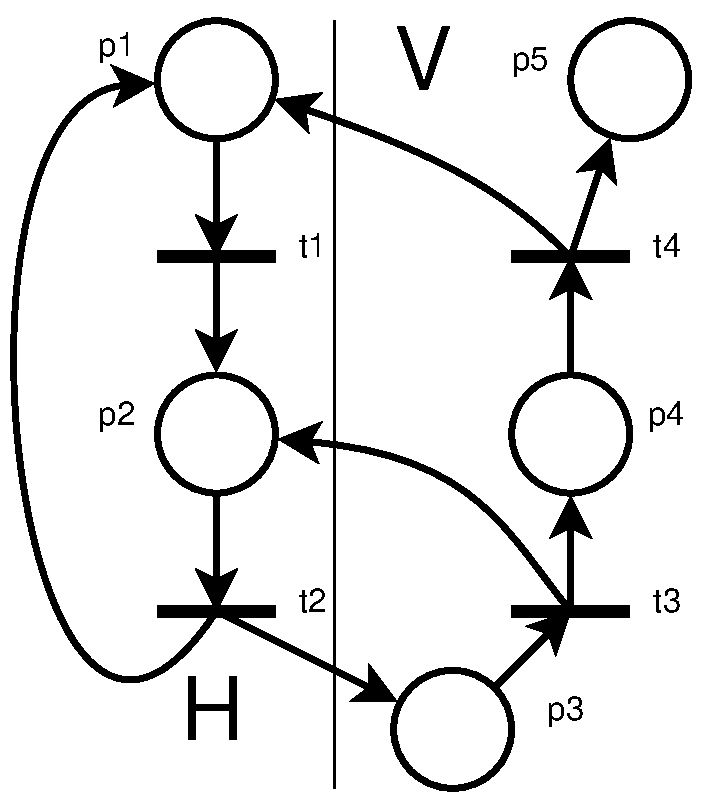
\includegraphics[width=0.3\textwidth]{Figures/EleccionSubredZonasInfluencia_2.eps}
\]



I want to occult the part marked with an H, so the result is this graphic

\[
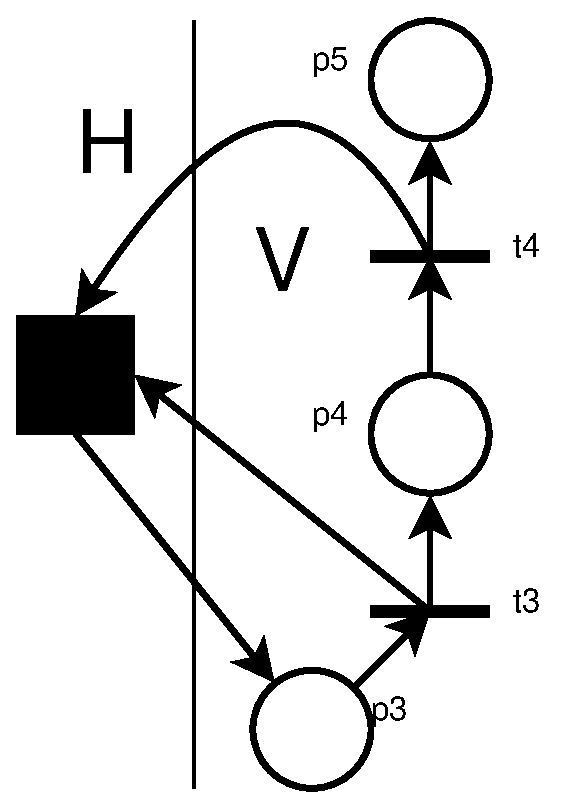
\includegraphics[width=0.25\textwidth]{Figures/OcultacionSubred_1.eps}
\]

And now, how can I maintain the H subnet information on the black box?
If I want to distribute  this Petri net I should send something more to that
people I want to access the hidden subnet. I have not found a way to embed
that information in the graphic so that some people can access it but other
people can't.
\end{example}

So this representation is useful in order to show at one sight the Petri
net structure, but I can't choose it  for my goals.
I have not been able to discover a way to show some people the hidden
information (the hidden subnet). However I will continue using it where a clear idea of the Petri structure
if necessary.

\subsection{Matrix representation}
This representation is very useful to study properties and evolution of a
Petri net, independently of its graphic representation.
As we have seen before (in chapter \ref{Chapter: Subnets}), we can reorder
rows and columns and define subnets
in the matrix.
\begin{example}[Matrix representation of a hidden subnet]
\label{ej:matrix_representation_hidden_subnet}
This is the matrix representation of the Petri net in the previous example
\ref{ej:graphic_representation_hidden_subnet}.
\[
\kbordermatrix{
   & t_1 & t_2 & t_3 & t_4\\
p_1& -1 &  1  &  0  &  1 \\
p_2&  1 & -1  &  1  &  0 \\
p_3&  0 &  1  & -1  &  0 \\
p_4&  0 &  0  &  1  & -1 \\
p_5&  0 &  0  &  0  &  1 \\
}
\]

As we can see before,  If I occult the part marked with an H, so the result is:
\[
\kbordermatrix{
   & t_1 &  t_2 & \vline &t_3 & t_4\\
p_1& \rule{0.15in}{0.15in} & \rule{0.15in}{0.15in} & \vline &  0  & 1 \\
p_2& \rule{0.15in}{0.15in} & \rule{0.15in}{0.15in} & \vline &  1  & 0 \\
\hline
p_3&  0 &  1  & \vline & -1  &  0 \\
p_4&  0 &  0  & \vline &  1  & -1 \\
p_5&  0 &  0  & \vline &  0  &  1 \\
}
\]

or this other one, grouping the places and transitions of the hidden subnet as seen in chapter \ref{Chapter: Subnets}
\[
\kbordermatrix{
    &  _                      & \vline & t_3 & t_4 \\
    & \rule{0.15in}{0.15in}   & \vline &  1  &  1  \\
\hline
p_3 &  1                      & \vline & -1  &  0  \\
p_4 &  0                      & \vline &  1  & -1  \\
p_5 &  0                      & \vline &  0  &  1  \\
}
\]


And now I have the same problems as in graphic mode: how can I keep  information
in the black box?
\end{example}

With this representation it is possible to study properties and it may be really important
as a complement to graphic mode. With both representations together, everyone has a clear idea of the Petri net structure and properties.  But I haven't
found a way to store information inside the black box. 

\subsection{Equation representation}
The third representation way for Petri nets is the equation representation.
Basically, transitions are selected and, for each one, the tokens of the places
connected to that transition are modified. This is very useful to compute
the evolution of a Petri net, choosing the transition fired.

However it is difficult to find a way for representing subnets with this
notation. And, of course, if a subnet cannot be represented, it cannot be
hidden. 

\begin{example}[Equation representation of a hidden subnet]
\label{ej:equation_representation_hidden_subnet}
Let's take again the Petri net from the previous examples \ref{ej:graphic_representation_hidden_subnet}.
This is It's equation representation:

\begin{scriptsize}
\begin{alltt}
if (p1>0) then
        p1 <- p1 - 1
        p2 <- p2 + 1
if (p2>0) then
        p2 <- p2 - 1
        p1 <- p1 + 1
        p3 <- p3 + 1
if (p3>0) then
        p3 <- p3 - 1
        p2 <- p2 + 1
        p4 <- p4 + 1
if (p4>0) then
        p4 <- p4 - 1
        p1 <- p1 + 1
        p5 <- p5 + 1
\end{alltt}
\end{scriptsize}

As we can see, we should hide several lines. In particular all that includes
places $p_1$ and $p_2$, resulting something like this (strikethrough text
would be part of the subnet):

\begin{scriptsize}
\begin{alltt}
\xout{if (p1>0) then}
        \xout{p1 <- p1 - 1}
        \xout{p2 <- p2 + 1}
\xout{if (p2>0) then}
        \xout{p2 <- p2 - 1}
        \xout{p1 <- p1 + 1}
        p3 <- p3 + 1
if (p3>0) then
        p3 <- p3 - 1
        \xout{p2 <- p2 + 1}
        p4 <- p4 + 1
if (p4>0) then
        p4 <- p4 - 1
        \xout{p1 <- p1 + 1}
        p5 <- p5 + 1
\end{alltt}
\end{scriptsize}

This is probably the strangest way to represent Petri nets and it is difficult
to define subnets over it.

\end{example}


I have tried to think about these ways of representation but, in my opinion, no one of them is suitable enough to represent subnets in a clear way than can be occulted. Because of that I have chosen the fourth representation, which is PNML, and that is explained in the next section. 

%----------------------------------------------------------------------------------------
%       SECTION 2
%----------------------------------------------------------------------------------------
\section{PNML. Petri Net Marked Language}

As I have explain in the Literature review in the chapter \ref{Chapter: LiteratureReview},
 PNML is a way to represent Petri nets as xml content.

The advantages over the other three representation ways described before
are clear. By one side, XML is a widely extended format to represent almost
everything. And not only that. XML is a robust technology free of errors
and it is really flexible. Its flexibility come from you can add any kind
of labels and functionality with a very little amount of work. Its robustness come from the strict
specification of the schemas declared to define completely the XML files    
that support. Once
the schema is defined, the XML files have a no way to get out of this definition,
so we can know if a XML file is correct given its schema. And this is not all. If you have an XML file, you can extract information to and complete it to create a schema for that file.  



Originally, with basic Petri nets, the structure of a Petri net was fully provided.
The only thing that is not supported in comparison with graphic mode is the graphical appearance of Petri nets: the position of nodes and
transitions was not
important, but with the arrival of High level Petri nets and Petri nets design
software, it is necessary to store this kind of information.

In this work, I am going to study only basic Petri nets, but
that concept and the method is easily exportable to other kind of nets, such as Symmetric nets and High Level Petri nets (that are representable in PNML
format too.)

\subsection{Scope}
The scope of this work in this section is basically bounded by the original
and basic Petri nets, that is:
\begin{itemize}
\item there are places, transitions and arcs between them
\item places can have tokens on them (but this does not  influence the hiding process)
\item transitions can be fired, but there is only one type of transition
(not messages, not time, etc.)
\end{itemize}

Furthermore, I am going to explain several concepts for a specific graphical
design of the Petri net (that will not influence the process either).

There are other options such as specific information for the design tool
that I am not going to discuss because the tools have no interest in this work 

\subsection{Description}
Petri Net Marked Language is an xml language created to represent Petri Nets. With this language we can take a Petri Net and store it into an xml file without loss of information.

One of the best properties of PNML is that, as it is an xml based schema,
it can be extended with more functionality extending the grammar.
Virtually, any extension over Petri nets can be translated into PNML in a logical and natural way.
Moreover, this extension is defined by Petri net type definition \cite{PNML-Billington2003483,PNML-iso/iec-15909-2:2011}.
 

In this case PNML hasn't got a way to represent subnets. There is something named \texttt{<page>} 
that is used to represent several nets in the same PNML file. But, by default,
a node inside a page cannot connect with a node of other page. So it cannot
be used as "subnets". So I am going to extend the language in order to get several goals:
\begin{enumerate}
\item Represent subnets of a Petri Net.
\item Include input and output interfaces for every subnet.
\end{enumerate}

As we can think, definition of several subnets of a Petri net is possible
and the connection over them are always through their respective interfaces.

\subsection{PNML grammar}

As PNML is an xml based language it has to be described by an schema that define the creation rules of the PNML representation of a Petri net.

The grammar is defined since 2009 and updated until
2012, which is the most recent revision.
I am not going to do and extensive explanation of all the possibilities
of the grammar, but the most important. As we can see later, anything we think is useful can be added to the process with little effort.
So I am going to study only the most basic elements of a Petri net. The rest of the element can be attached later with facility. 

\subsubsection{PNML basics}

In this section I am going to explain several characteristics of PNML files.
With these explanations it is going to be easier the understanding of PNML
structure.

First of all, as PNML files are xml files, there several things to know:

\begin{enumerate}
\item 
  A xml file normally starts with a line defining some characteristics of
  the file, like the version and the encoding type. It has an aspect like
  this\footnote{For clarity, in the following examples, this line can be deleted.}: 

\begin{lstlisting}
<?xml version="1.0" encoding="utf-8"?>
\end{lstlisting}
  
 
\item
  A root node must exist.
  In this case, the root node is \texttt{<pnml>}.
  So every PNML files has to start with the tag \texttt{<pnml>} and end with the tag \texttt{</pnml>}.
Below this tag, there is a new tag \texttt{<net>} that can contain
  \begin{itemize}
  \item Type: the type of the Petri net as an attribute. In this case, as
    I  am going to study only Place/Transition nets, it will  be \texttt{ptnet}
  \item Name of the net: New tag \texttt{<name><text>...</text></name>}
  \item Pages: one page is an invention to store several Petri nets inside
  an unique PNML file, but usually there is only one page for file. It is
  nested inside a \texttt{<page>} tag.
  \end{itemize}
  \item
  Each element in PNML has to have a unique id inside the net to be identified
unambiguously. So there cannot
  be two elements with the same id.
\end{enumerate}

 

With this three observations, we can have an idea about how a PNML file
is structured:  

 
\begin{lstlisting}[label=pnml_net_page,caption=Example of general PNML file]
<?xml version="1.0" encoding="utf-8"?>
<pnml>
  <net id="myNet" type="http://www.pnml.org/version-2009/grammar/ptnet">
    <name>
      <text> My new net </text>
    </name>
    <page id="page1">
      .......
    </page>
  </net>
</pnml>
\end{lstlisting}

Once this structure is defined, I am going to explain the next stage, that
is the most important one in this work. 

\subsubsection{Places, transitions and arcs in PNML}

As Petri nets has three main elements, places, transitions
and arcs, and PNML has them too. These three elements have several things in common in an PNML file:
\begin{itemize}
  \item They are all nested in a page tag


  \item Places and transitions (not arcs) can contain a tag \texttt{<name>} with its name. This tag has been defined before for the name of the net. It
can store information about the text of the name and the graphical position
of this label in this way:
\begin{lstlisting}
<name>
  <text> Element Name </text>
  <graphics>
    <offset x="22" y="-10"/>
  </graphics>
</name>
\end{lstlisting}
   \item They can contain a tag \texttt{<graphics>} with information about its position and dimension:
\begin{lstlisting}
<graphics>
  <position x="100" y="200"/>
  <dimension x="40" y="40"/>
</graphics>
\end{lstlisting}
\end{itemize}


These are the common properties of places, transitions and arcs. Now let's
go on the particular characteristics of each one of them.

Places are represented with the tag \texttt{<place>} and the can have a marking with the label \texttt{<initialMarking>}.
Here we have an example of a place with two tokens in PNML: 

\begin{lstlisting}[label=pmnl_place,caption=PNML representation
for places]
<place id="p1">
  <name>
    <text> Place number one </text>
    <graphics>
      <offset x="130" y="130"/>
    </graphics>
  </name>
  <graphics>
    <position x="130" y="90"/>
    <dimension x="40" y="40"/>
  </graphics>
  <initialMarking>
    <text> 2 </text>
  </initialMarking>
</place>
\end{lstlisting}

Transitions are represented with the tag \texttt{<transition>}.
This is an example of a transition in PNML: 

\begin{lstlisting}[label=pmnl_transition,caption=PNML representation
for transitions]
<transition id="t1">
  <name>
    <text> Transition number one </text>
    <graphics>
      <offset x="270" y="140"/>
    </graphics>
  </name>
  <graphics>
    <position x="270" y="100"/>
    <dimension x="40" y="40"/>
  </graphics>
</transition>
\end{lstlisting}

Arcs are represented with the tag \texttt{<arc>}. Arc
have to have a source and a target, which are defined by the attributes \texttt{source} and \texttt{target} that have to point to a transition and a place, identified
by their id. Furthermore, the arc weight can be fixed by the \texttt{<inscription>}
 tag.
If the weight is one, the tag inscription is not necessary because this is
the default value. This is an example of the arc with weight 3 that connects the place and the
transition of the previous examples in PNML: 

\begin{lstlisting}[label=pmnl_arc,caption=PNML representation
for arcs]
<arc id="a1" source="p1" target="t1">
  <inscription> 3 </inscription>
</arc>
\end{lstlisting}

\newpage
If we take the last examples all together, we can represent the following Petri net:

\[
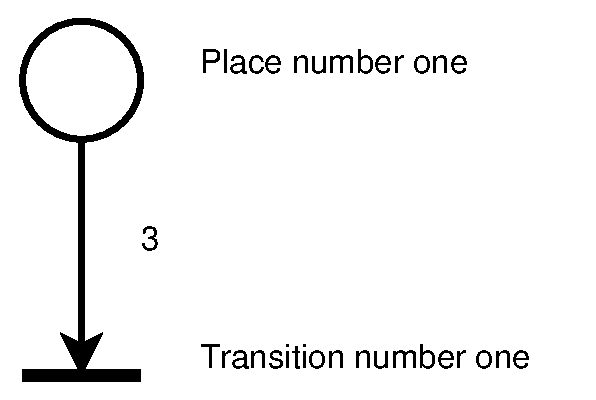
\includegraphics[width=0.3\textwidth]{Figures/PNML-RdPBasicaCompleta.eps}
\]

\begin{lstlisting}[label=pmnl_complete_representation,caption=Complete PNML representation
for a basic Petri net]
<?xml version="1.0" encoding="utf-8"?>
<pnml>
  <net id="myNet" type="http://www.pnml.org/version-2009/grammar/ptnet">
    <name>
      <text> My new net </text>
    </name>
    <page id="page1">
      <place id="p1">
        <name>
          <text> Place number one </text>
          <graphics>
            <offset x="130" y="130"/>
          </graphics>
        </name>
        <graphics>
          <position x="130" y="90"/>
          <dimension x="40" y="40"/>
        </graphics>
        <initialMarking>
          <text> 2 </text>
        </initialMarking>
      </place>
      <transition id="t1">
        <name>
          <text> Transition number one </text>
          <graphics>
            <offset x="270" y="140"/>
          </graphics>
        </name>
        <graphics>
          <position x="270" y="100"/>
          <dimension x="40" y="40"/>
        </graphics>
      </transition>
      <arc id="a1" source="p1" target="t1">
        <inscription> 3 </inscription>
      </arc>
    </page>
  </net>
</pnml>
\end{lstlisting}

For clarity, I am going to obviate several options. I am not going to put the graphic information and the names, but the id. So this last example is as follows:

\[
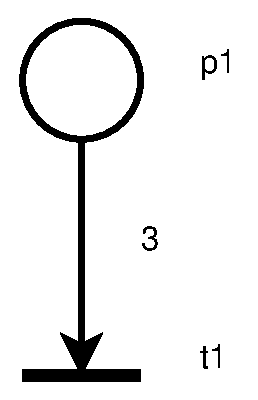
\includegraphics[width=0.11\textwidth]{Figures/PNML-RdPBasica.eps}
\]

\begin{lstlisting}[label=pmnl_basic_representation,caption=Basic PNML representation
for a basic Petri net]
<?xml version="1.0" encoding="utf-8"?>
<pnml>
  <net id="myNet" type="http://www.pnml.org/version-2009/grammar/ptnet">
    <page id="page1">
      <place id="p1">
        <initialMarking>
          <text> 2 </text>
        </initialMarking>
      </place>
      <transition id="t1"/>
      <arc id="a1" source="p1" target="t1">
        <inscription> 3 </inscription>
      </arc>
    </page>
  </net>
</pnml>
\end{lstlisting}


I think that this last listing is clear enough to understand the rest of
the process. But not only that. For even more clarity, the tags \texttt{<?xml>}, \texttt{<pnml>}, \texttt{<net>} and \texttt{<page>} are going to be obviated
too. So in many of the later examples they will not be present. Applying
this criterium, the listing \ref{pmnl_basic_representation} change to:

\begin{lstlisting}[label=pmnl_simplified_representation,caption=Simplified PNML representation
for a basic Petri net]
<place id="p1">
  <initialMarking>
    <text> 2 </text>
 </initialMarking>
</place>
<transition id="t1"/>
<arc id="a1" source="p1" target="t1">
  <inscription> 3 </inscription>
</arc>
\end{lstlisting}








\subsection{PNML examples}

Now I am going to present some Petri nets in format PNML, in order to get
used to work with this type of representation. As I said before, one thing to have in mind
is that, in PNML, each element can have a name (tag \texttt{<name>}) and a position
(tag \texttt{<graphics>}).  Even the
tag \texttt{<name>} itself can have its own \texttt{<graphics>} inside. As
a result, a PNML representation grows in size with lots and lots of elements
\texttt{<graphics>}, although they have only information about the elements
position: they have no influence (at first) in the net behaviour.

So in all of these following Petri nets examples,
I am going to eliminate, at least, the information about the exact situation of the elements, keeping only the internal structure of the net,
in order to be shorter and clearer. So all the tags \texttt{<graphics>} are going to
be deleted.

Anyway, obviously, in a real case, this information can be stored and processed
with no problem. It is the very nature of the net who is going to demand the exact information to be processed. 

\subsubsection{The dining philosophers}

One famous example of Petri net is the model of the dining philosophers
problem.
This problem, formulated by Edsger Dijkstra in 1965 says:

"Five silent philosophers sit at a round table with bowls of spaghetti. Forks are placed between each pair of adjacent philosophers.

Each philosopher must alternately think and eat. However, a philosopher can only eat spaghetti when he has both left and right forks. Each fork can be held by only one philosopher and so a philosopher can use the fork only if it is not being used by another philosopher. After he finishes eating, he needs to put down both forks so they become available to others. A philosopher can take the fork on his right or the one on his left as they become available, but cannot start eating before getting both of them.

Eating is not limited by the remaining amounts of spaghetti or stomach space; an infinite supply is assumed.

The problem is how to design a discipline of behavior (a concurrent algorithm) such that each philosopher will not starve; i.e., can forever continue to alternate between eating and thinking, assuming that any philosopher cannot know when others may want to eat or think."

It is a classic problem
modelled by the  well known Petri net in figure \ref{fig:PNML_dining_philosofers}:


\begin{figure}[htbp]
\[
\includegraphics[width=1\textwidth]{Figures/DiningPhilosophers.eps}
\]
\rule{35em}{0.5pt}
 \caption{Dining philosophers Petri net}
 \label{fig:PNML_dining_philosofers}
\end{figure} 

Here are the descriptions of each element:
\begin{itemize}
\item M1..M5: philosophers waiting
\item C1..C5: forks
\item E1..E5: philosopher eating
\item t1..t5 - r1..r5: transitions


\end{itemize}

Obviating the graphics information about the exact position of the elements,
the PNML content that represents this Petri net is as follows: \note{This PNML content is in two columns for space reasons}
\begin{multicols}{2}
\begin{lstlisting}[basicstyle=\ttfamily\tiny]
<?xml version="1.0" encoding="UTF-8"?>
<pnml
    xmlns="http://www.pnml.org/version-2009/grammar/pnml">
  <net id="5Philo"
      type="http://www.pnml.org/version-2009/grammar/ptnet">
    <page id="page1">
      <place id="p7">
        <name>
          <text>E2</text>
        </name>
      </place>
      <place id="p6">
        <name>
          <text>C2</text>
        </name>
        <initialMarking>
          <text>1</text>
        </initialMarking>
      </place>
      <place id="p5">
        <name>
          <text>M2</text>
        </name>
        <initialMarking>
          <text>1</text>
        </initialMarking>
      </place>
      <place id="p4">
        <name>
          <text>E1</text>
        </name>
      </place>
      <place id="p3">
        <name>
          <text>C1</text>
        </name>
        <initialMarking>
          <text>1</text>
        </initialMarking>
      </place>
      <place id="p2">
        <name>
          <text>M1</text>
        </name>
        <initialMarking>
          <text>1</text>
        </initialMarking>
      </place>
      <place id="p1">
        <name>
          <text>C5</text>
        </name>
        <initialMarking>
          <text>1</text>
        </initialMarking>
      </place>
      <place id="p10">
        <name>
          <text>E3</text>
        </name>
      </place>
      <place id="p9">
        <name>
          <text>C3</text>
        </name>
        <initialMarking>
          <text>1</text>
        </initialMarking>
      </place>
      <place id="p8">
        <name>
          <text>M3</text>
        </name>
        <initialMarking>
          <text>1</text>
        </initialMarking>
      </place>
      <place id="p16">
        <name>
          <text>E5</text>
        </name>
      </place>
      <place id="p14">
        <name>
          <text>M5</text>
        </name>
        <initialMarking>
          <text>1</text>
        </initialMarking>
      </place>
      <place id="p13">
        <name>
          <text>E4</text>
        </name>
      </place>
      <place id="p12">
        <name>
          <text>C4</text>
        </name>
        <initialMarking>
          <text>1</text>
        </initialMarking>
      </place>
      <place id="p11">
        <name>
          <text>M4</text>
        </name>
        <initialMarking>
          <text>1</text>
        </initialMarking>
      </place>
      <transition id="t3">
        <name>
          <text>t3</text>
        </name>
      </transition>
      <transition id="t2">
        <name>
          <text>t2</text>
        </name>
      </transition>
      <transition id="t1">
        <name>
          <text>t1</text>
        </name>
      </transition>
      <transition id="t10">
        <name>
          <text>r4</text>
        </name>
      </transition>
      <transition id="t11">
        <name>
          <text>r5</text>
        </name>
      </transition>
      <transition id="t4">
        <name>
          <text>t4</text>
        </name>
      </transition>
      <transition id="t5">
        <name>
          <text>t5</text>
        </name>
      </transition>
      <transition id="t7">
        <name>
          <text>r1</text>
        </name>
      </transition>
      <transition id="t8">
        <name>
          <text>r2</text>
        </name>
      </transition>
      <transition id="t9">
        <name>
          <text>r3</text>
        </name>
      </transition>
      <arc id="a41" source="p12" target="t5"/>
      <arc id="a20" source="p10" target="t9"/>
      <arc id="a16" source="t8" target="p3"/>
      <arc id="a9" source="t7" target="p1"/>
      <arc id="a17" source="t8" target="p6"/>
      <arc id="a14" source="p6" target="t2"/>
      <arc id="a15" source="p3" target="t2"/>
      <arc id="a12" source="p7" target="t8"/>
      <arc id="a13" source="t8" target="p5"/>
      <arc id="a10" source="p5" target="t2"/>
      <arc id="a11" source="t2" target="p7"/>
      <arc id="a35" source="t5" target="p16"/>
      <arc id="a34" source="p14" target="t5"/>
      <arc id="a2" source="p2" target="t1"/>
      <arc id="a33" source="t10" target="p12"/>
      <arc id="a3" source="t1" target="p4"/>
      <arc id="a32" source="t10" target="p9"/>
      <arc id="a4" source="p4" target="t7"/>
      <arc id="a5" source="t7" target="p2"/>
      <arc id="a38" source="t11" target="p12"/>
      <arc id="a6" source="p1" target="t1"/>
      <arc id="a37" source="t11" target="p14"/>
      <arc id="a7" source="p3" target="t1"/>
      <arc id="a18" source="p8" target="t3"/>
      <arc id="a19" source="t3" target="p10"/>
      <arc id="a8" source="t7" target="p3"/>
      <arc id="a36" source="p16" target="t11"/>
      <arc id="a51" source="t11" target="p1"/>
      <arc id="a52" source="p1" target="t5"/>
      <arc id="a31" source="p12" target="t4"/>
      <arc id="a30" source="p9" target="t4"/>
      <arc id="a25" source="t9" target="p9"/>
      <arc id="a26" source="p11" target="t4"/>
      <arc id="a27" source="t4" target="p13"/>
      <arc id="a28" source="p13" target="t10"/>
      <arc id="a21" source="t9" target="p8"/>
      <arc id="a22" source="p6" target="t3"/>
      <arc id="a23" source="p9" target="t3"/>
      <arc id="a24" source="t9" target="p6"/>
      <arc id="a29" source="t10" target="p11"/>
    </page>
  </net>
</pnml>
\end{lstlisting}
\end{multicols}

\subsubsection{Mengchu Zhou benmarch}
This other example is a famous Petri net modelled by Mengchu Zhou. The graphical
representation is the figure \ref{fig:PNML_MengchuZhou}.

Again, this is the PNML representation, obviating the data associated to
graphical position and labels, in order to be clearer 
\begin{figure}[htbp]
\[
\includegraphics[width=1\textwidth]{Figures/MengchuZhou.eps}
\]
\rule{35em}{0.5pt}
 \caption{Mengchu Zhou's Petri net}
 \label{fig:PNML_MengchuZhou}
\end{figure}

\begin{multicols}{2}
\begin{lstlisting}[basicstyle=\ttfamily\tiny]
<?xml version="1.0" encoding="UTF-8"?>
<pnml
    xmlns="http://www.pnml.org/version-2009/grammar/pnml">
  <net id="MengchuZhou"
      type="http://www.pnml.org/version-2009/grammar/ptnet">
    <page id="page1">
      <place id="p5"/>
      <place id="p4"/>
      <place id="p3"/>
      <place id="p2"/>
      <place id="p1"/>
      <place id="p40"/>
      <place id="p41"/>
      <place id="p42"/>
      <place id="p43"/>
      <place id="p45"/>
      <place id="p44"/>
      <place id="p47"/>
      <place id="p46"/>
      <place id="p49"/>
      <place id="p48"/>
      <place id="p31"/>
      <place id="p32"/>
      <place id="p30"/>
      <place id="p36"/>
      <place id="p35"/>
      <place id="p34"/>
      <place id="p33"/>
      <place id="p39"/>
      <place id="p38"/>
      <place id="p37"/>
      <place id="p20"/>
      <place id="p21"/>
      <place id="p27"/>
      <place id="p26"/>
      <place id="p29"/>
      <place id="p28"/>
      <place id="p23"/>
      <place id="p22"/>
      <place id="p25"/>
      <place id="p24"/>
      <place id="p99"/>
      <place id="p18"/>
      <place id="p17"/>
      <place id="p16"/>
      <place id="p90"/>
      <place id="p15"/>
      <place id="p14"/>
      <place id="p13"/>
      <place id="p12"/>
      <place id="p11"/>
      <place id="p95"/>
      <place id="p96"/>
      <place id="p97"/>
      <place id="p98"/>
      <place id="p91"/>
      <place id="p92"/>
      <place id="p93"/>
      <place id="p94"/>
      <place id="p19"/>
      <place id="p88"/>
      <place id="p89"/>
      <place id="p83"/>
      <place id="p82"/>
      <place id="p81"/>
      <place id="p87"/>
      <place id="p86"/>
      <place id="p85"/>
      <place id="p84"/>
      <place id="p111"/>
      <place id="p110"/>
      <place id="p113"/>
      <place id="p112"/>
      <place id="p114"/>
      <place id="p109"/>
      <place id="p108"/>
      <place id="p107"/>
      <place id="p102"/>
      <place id="p101"/>
      <place id="p100"/>
      <place id="p106"/>
      <place id="p105"/>
      <place id="p104"/>
      <place id="p103"/>
      <place id="p50"/>
      <transition id="t33"/>
      <transition id="t34"/>
      <transition id="t35"/>
      <transition id="t36"/>
      <transition id="t30"/>
      <transition id="t31"/>
      <transition id="t32"/>
      <transition id="t37"/>
      <transition id="t38"/>
      <transition id="t20"/>
      <transition id="t21"/>
      <transition id="t24"/>
      <transition id="t25"/>
      <transition id="t22"/>
      <transition id="t23"/>
      <transition id="t28"/>
      <transition id="t29"/>
      <transition id="t26"/>
      <transition id="t10"/>
      <transition id="t11"/>
      <transition id="t12"/>
      <transition id="t13"/>
      <transition id="t14"/>
      <transition id="t15"/>
      <transition id="t16"/>
      <transition id="t17"/>
      <transition id="t18"/>
      <transition id="t19"/>
      <transition id="t71"/>
      <transition id="t72"/>
      <transition id="t70"/>
      <transition id="t76"/>
      <transition id="t75"/>
      <transition id="t74"/>
      <transition id="t73"/>
      <transition id="t79"/>
      <transition id="t78"/>
      <transition id="t77"/>
      <transition id="t80"/>
      <transition id="t81"/>
      <transition id="t82"/>
      <transition id="t4"/>
      <transition id="t9"/>
      <transition id="t3"/>
      <transition id="t2"/>
      <transition id="t1"/>
      <transition id="t61"/>
      <transition id="t67"/>
      <transition id="t66"/>
      <transition id="t69"/>
      <transition id="t68"/>
      <transition id="t63"/>
      <transition id="t62"/>
      <transition id="t65"/>
      <transition id="t64"/>
      <arc id="a63" source="p27" target="t24"/>
      <arc id="a64" source="p43" target="t37"/>
      <arc id="a61" source="t22" target="p27"/>
      <arc id="a62" source="t23" target="p27"/>
      <arc id="a60" source="t22" target="p25"/>
      <arc id="a120" source="p82" target="t62"/>
      <arc id="a121" source="p82" target="t69"/>
      <arc id="a123" source="p81" target="t62"/>
      <arc id="a122" source="p91" target="t69"/>
      <arc id="a125" source="t70" target="p88"/>
      <arc id="a59" source="t23" target="p30"/>
      <arc id="a124" source="t64" target="p95"/>
      <arc id="a58" source="t21" target="p28"/>
      <arc id="a127" source="p97" target="t24"/>
      <arc id="a57" source="t25" target="p28"/>
      <arc id="a126" source="p96" target="t15"/>
      <arc id="a56" source="p28" target="t19"/>
      <arc id="a129" source="t24" target="p99"/>
      <arc id="a55" source="p28" target="t17"/>
      <arc id="a128" source="t15" target="p98"/>
      <arc id="a54" source="p26" target="t19"/>
      <arc id="a72" source="p36" target="t33"/>
      <arc id="a73" source="p47" target="t28"/>
      <arc id="a74" source="t28" target="p45"/>
      <arc id="a75" source="p45" target="t38"/>
      <arc id="a110" source="p84" target="t65"/>
      <arc id="a70" source="p42" target="t31"/>
      <arc id="a71" source="t31" target="p36"/>
      <arc id="a119" source="p87" target="t62"/>
      <arc id="a114" source="t64" target="p83"/>
      <arc id="a113" source="t70" target="p83"/>
      <arc id="a69" source="t35" target="p42"/>
      <arc id="a112" source="p90" target="t70"/>
      <arc id="a111" source="t65" target="p90"/>
      <arc id="a118" source="p87" target="t69"/>
      <arc id="a66" source="p44" target="t36"/>
      <arc id="a117" source="t65" target="p87"/>
      <arc id="a65" source="t37" target="p44"/>
      <arc id="a116" source="t61" target="p87"/>
      <arc id="a68" source="p41" target="t35"/>
      <arc id="a115" source="p83" target="t68"/>
      <arc id="a67" source="t36" target="p41"/>
      <arc id="a140" source="p104" target="t76"/>
      <arc id="a141" source="t76" target="p106"/>
      <arc id="a142" source="t76" target="p107"/>
      <arc id="a143" source="t76" target="p108"/>
      <arc id="a41" source="p30" target="t20"/>
      <arc id="a42" source="t20" target="p31"/>
      <arc id="a40" source="p21" target="t23"/>
      <arc id="a9" source="p16" target="t10"/>
      <arc id="a149" source="p105" target="t78"/>
      <arc id="a35" source="t17" target="p23"/>
      <arc id="a1" source="p1" target="t1"/>
      <arc id="a148" source="p109" target="t77">
        <inscription>
          <text>2</text>
        </inscription>
      </arc>
      <arc id="a34" source="p24" target="t17"/>
      <arc id="a2" source="t1" target="p2"/>
      <arc id="a33" source="t18" target="p24"/>
      <arc id="a3" source="p2" target="t2"/>
      <arc id="a32" source="p25" target="t18"/>
      <arc id="a4" source="t2" target="p3"/>
      <arc id="a145" source="p106" target="t77">
        <inscription>
          <text>2</text>
        </inscription>
      </arc>
      <arc id="a39" source="t25" target="p21"/>
      <arc id="a5" source="p3" target="t3"/>
      <arc id="a144" source="t76" target="p109"/>
      <arc id="a38" source="p22" target="t25"/>
      <arc id="a6" source="t3" target="p4"/>
      <arc id="a147" source="p108" target="t77">
        <inscription>
          <text>3</text>
        </inscription>
      </arc>
      <arc id="a37" source="t16" target="p22"/>
      <arc id="a7" source="p4" target="t4"/>
      <arc id="a146" source="p107" target="t77"/>
      <arc id="a36" source="p23" target="t16"/>
      <arc id="a8" source="t4" target="p5"/>
      <arc id="a131" source="p101" target="t68"/>
      <arc id="a132" source="t30" target="p102"/>
      <arc id="a130" source="p100" target="t30"/>
      <arc id="a50" source="p35" target="t17"/>
      <arc id="a51" source="p29" target="t17"/>
      <arc id="a53" source="p29" target="t19"/>
      <arc id="a44" source="t19" target="p32"/>
      <arc id="a139" source="t74" target="p105"/>
      <arc id="a43" source="p31" target="t19"/>
      <arc id="a138" source="t74" target="p104"/>
      <arc id="a46" source="t26" target="p33"/>
      <arc id="a137" source="p103" target="t75"/>
      <arc id="a45" source="p32" target="t26"/>
      <arc id="a136" source="p102" target="t74"/>
      <arc id="a48" source="t21" target="p34"/>
      <arc id="a135" source="p99" target="t73"/>
      <arc id="a47" source="p33" target="t21"/>
      <arc id="a134" source="p98" target="t72"/>
      <arc id="a133" source="t68" target="p103"/>
      <arc id="a49" source="p34" target="t22"/>
      <arc id="a98" source="t69" target="p86"/>
      <arc id="a99" source="p86" target="t66"/>
      <arc id="a20" source="p17" target="t2"/>
      <arc id="a161" source="t80" target="p113"/>
      <arc id="a160" source="t79" target="p39"/>
      <arc id="a163" source="t82" target="p82"/>
      <arc id="a162" source="p113" target="t82"/>
      <arc id="a165" source="t33" target="p19"/>
      <arc id="a164" source="t82" target="p101"/>
      <arc id="a166" source="t74" target="p48"/>
      <arc id="a16" source="t9" target="p12"/>
      <arc id="a167" source="t32" target="p20"/>
      <arc id="a17" source="p12" target="t12"/>
      <arc id="a168" source="t74" target="p38"/>
      <arc id="a14" source="t10" target="p13"/>
      <arc id="a169" source="t64" target="p35"/>
      <arc id="a15" source="p13" target="t9"/>
      <arc id="a12" source="t11" target="p14"/>
      <arc id="a13" source="p14" target="t10"/>
      <arc id="a10" source="p16" target="t2"/>
      <arc id="a11" source="p15" target="t11"/>
      <arc id="a18" source="t12" target="p11"/>
      <arc id="a19" source="p17" target="t10"/>
      <arc id="a150" source="t75" target="p100"/>
      <arc id="a31" source="p18" target="t15"/>
      <arc id="a30" source="t14" target="p15"/>
      <arc id="a154" source="t79" target="p111"/>
      <arc id="a153" source="p110" target="t79"/>
      <arc id="a152" source="t72" target="p97"/>
      <arc id="a151" source="t78" target="p96"/>
      <arc id="a157" source="p112" target="t81"/>
      <arc id="a25" source="t13" target="p18"/>
      <arc id="a26" source="t14" target="p18"/>
      <arc id="a155" source="p111" target="t80"/>
      <arc id="a27" source="p19" target="t2"/>
      <arc id="a156" source="t73" target="p112"/>
      <arc id="a28" source="p20" target="t10"/>
      <arc id="a21" source="t12" target="p17"/>
      <arc id="a22" source="t4" target="p17"/>
      <arc id="a159" source="t81" target="p110"/>
      <arc id="a23" source="p11" target="t13"/>
      <arc id="a24" source="p5" target="t14"/>
      <arc id="a29" source="t13" target="p1"/>
      <arc id="a76" source="t38" target="p46"/>
      <arc id="a77" source="p46" target="t34"/>
      <arc id="a78" source="t34" target="p50"/>
      <arc id="a79" source="p50" target="t29"/>
      <arc id="a80" source="t29" target="p49"/>
      <arc id="a82" source="p39" target="t36"/>
      <arc id="a81" source="p49" target="t32"/>
      <arc id="a84" source="p38" target="t38"/>
      <arc id="a83" source="p39" target="t38"/>
      <arc id="a86" source="p40" target="t36"/>
      <arc id="a85" source="p48" target="t36"/>
      <arc id="a102" source="t61" target="p89"/>
      <arc id="a89" source="t29" target="p40"/>
      <arc id="a103" source="p89" target="t64"/>
      <arc id="a100" source="t66" target="p85"/>
      <arc id="a87" source="p40" target="t38"/>
      <arc id="a101" source="p85" target="t61"/>
      <arc id="a88" source="t31" target="p40"/>
      <arc id="a106" source="p93" target="t62"/>
      <arc id="a107" source="t62" target="p94"/>
      <arc id="a104" source="p95" target="t71"/>
      <arc id="a105" source="t71" target="p93"/>
      <arc id="a108" source="p94" target="t67"/>
      <arc id="a173" source="t77" target="p114"/>
      <arc id="a109" source="t67" target="p84"/>
      <arc id="a172" source="t70" target="p26"/>
      <arc id="a171" source="t74" target="p81"/>
      <arc id="a170" source="t74" target="p91"/>
      <arc id="a93" source="t32" target="p43"/>
      <arc id="a92" source="p37" target="t30"/>
      <arc id="a91" source="t33" target="p37"/>
      <arc id="a90" source="t32" target="p37"/>
      <arc id="a97" source="p92" target="t69"/>
      <arc id="a96" source="t63" target="p92"/>
      <arc id="a95" source="p88" target="t63"/>
      <arc id="a94" source="t33" target="p47"/>
    </page>
  </net>
</pnml>
\end{lstlisting}
\end{multicols}


\subsubsection{Abstract example}
This last triple example is going to be the base of some other future examples.
It is based on Latorre's PhD \cite{G-Latorre2012PhD} and represent three nets. This example will be used later for the other purposes of this thesis.
I introduced these nets because they are quite simple and  the examples will
be very clear.
These nets are shown in the figure \ref{fig:Petri_net_examples}   

\begin{figure}[htbp]
\centering
\[
 \begin{matrix} 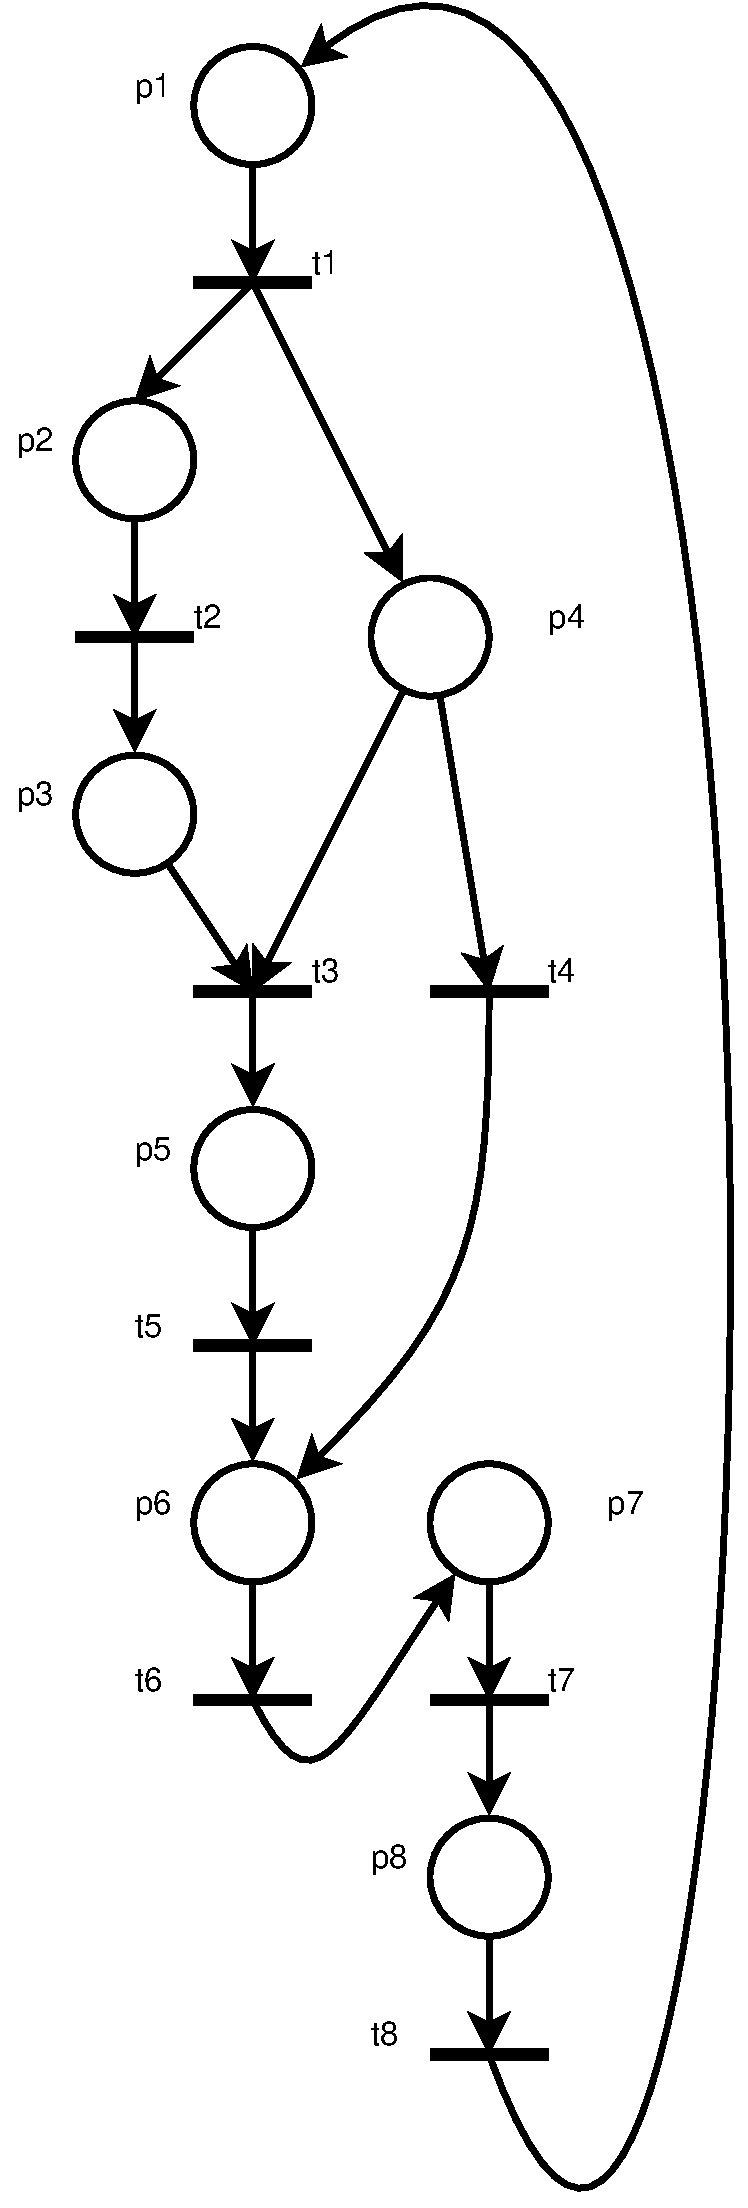
\includegraphics[width=0.2\textwidth]{Figures/PNML-Latorre_1.eps}\\a)\end{matrix}
  \ \ \ \ \ \ 
 \begin{matrix}  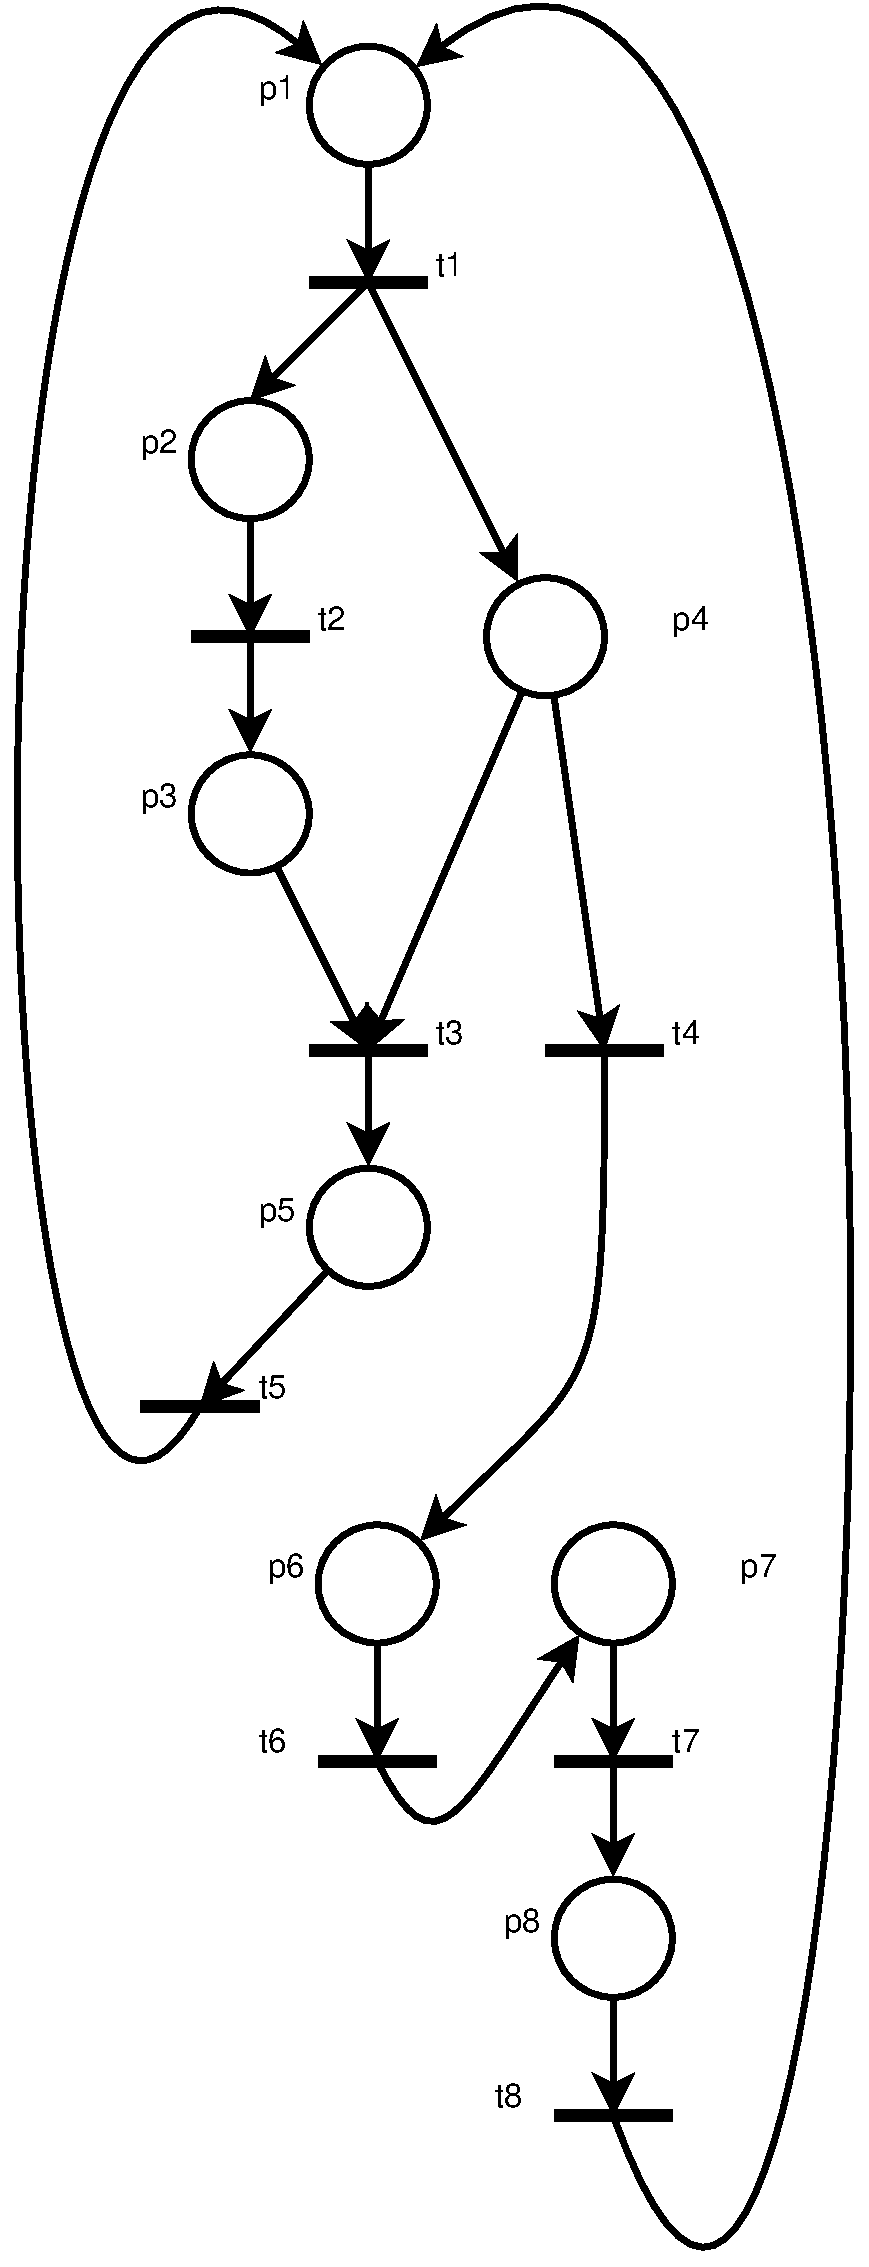
\includegraphics[width=0.23\textwidth]{Figures/PNML-Latorre_2.eps}\\b)\end{matrix}
  \ \ \ \ \ \ 
 \begin{matrix}  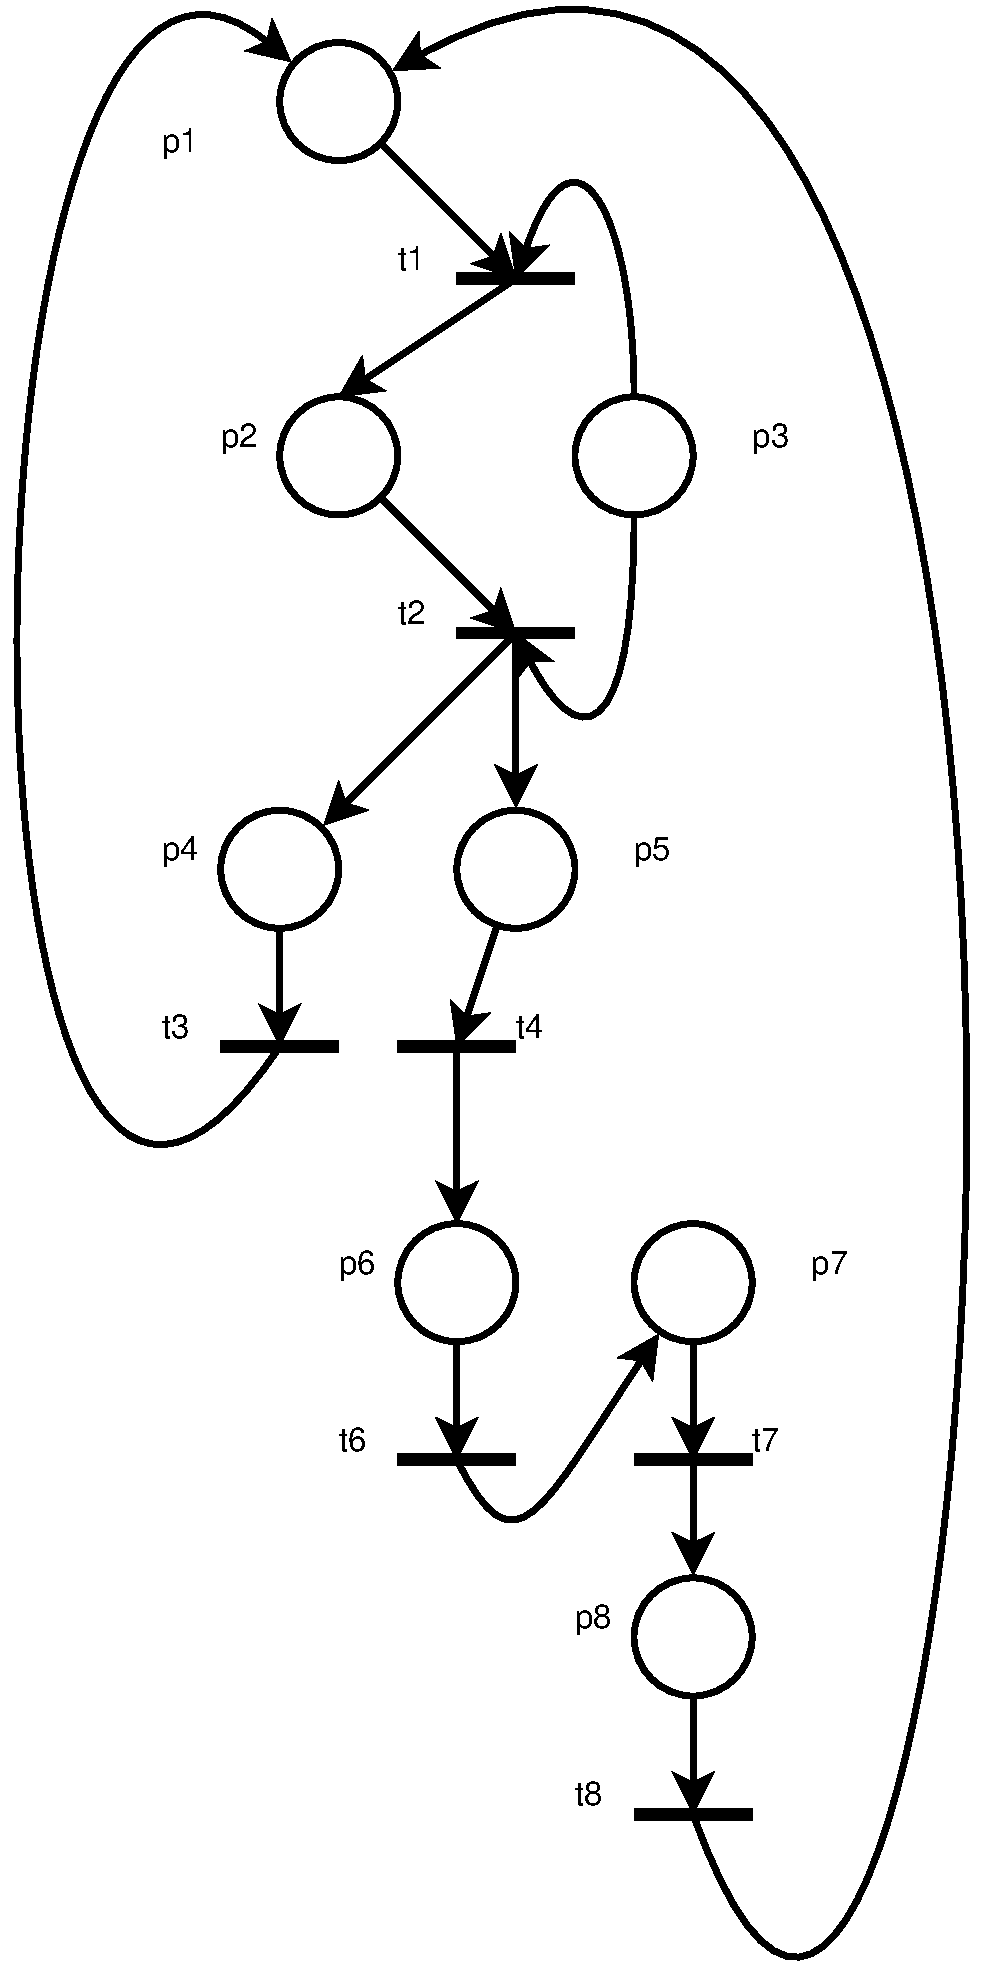
\includegraphics[width=0.3\textwidth]{Figures/PNML-Latorre_3.eps}\\c)\end{matrix}
\]
\rule{35em}{0.5pt}
 \caption{Three example Petri nets}
 \label{fig:Petri_net_examples} 
\end{figure}

The PNML representation of the a) net is:


\begin{lstlisting}
<?xml version="1.0" encoding="UTF-8"?>
<pnml
    xmlns="http://www.pnml.org/version-2009/grammar/pnml">
  <net id="latorre1"
      type="http://www.pnml.org/version-2009/grammar/ptnet">
    <page id="page1">
      <subnet id="N1">
        <content id="N1_content">
        </content>
      </subnet>
      <subnet id="N2">
        <content id="N2_content">
        </content>
      </subnet>
      <place id="p1"/>
      <place id="p2"/>
      <place id="p3"/>
      <place id="p4"/>
      <place id="p5"/>
      <place id="p6"/>
      <place id="p7"/>
      <place id="p8"/>
      <transition id="t1"/>
      <transition id="t2"/>
      <transition id="t3"/>
      <transition id="t4"/>
      <transition id="t5"/>
      <transition id="t6"/>
      <transition id="t7"/>
      <transition id="t8"/>
      <arc id="a1" source="p1" target="t1"/>
      <arc id="a2" source="t1" target="p2"/>
      <arc id="a3" source="p2" target="t2"/>
      <arc id="a4" source="t2" target="p3"/>
      <arc id="a5" source="t1" target="p4"/>
      <arc id="a6" source="p3" target="t3"/>
      <arc id="a7" source="p4" target="t4"/>
      <arc id="a8" source="p4" target="t3"/>
      <arc id="a9" source="t3" target="p5"/>
      <arc id="a10" source="p5" target="t5"/>
      <arc id="a11" source="t5" target="p6"/>
      <arc id="a12" source="p6" target="t6"/>
      <arc id="a13" source="t6" target="p7"/>
      <arc id="a14" source="p7" target="t7"/>
      <arc id="a15" source="t7" target="p8"/>
      <arc id="a16" source="p8" target="t8"/>
      <arc id="a17" source="t8" target="p1"/>
      <arc id="a18" source="t4" target="p6"/>
    </page>
  </net>
</pnml>
\end{lstlisting}


The PNML representation of the b) net is:


\begin{lstlisting}
<?xml version="1.0" encoding="UTF-8"?>
<pnml
    xmlns="http://www.pnml.org/version-2009/grammar/pnml">
  <net id="latorre2" 
      type="http://www.pnml.org/version-2009/grammar/ptnet">
    <page id="page1">
      <place id="p1"/>
      <place id="p2"/>
      <place id="p3"/>
      <place id="p4"/>
      <place id="p5"/>
      <place id="p6"/>
      <place id="p7"/>
      <place id="p8"/>
      <transition id="t1"/>
      <transition id="t2"/>
      <transition id="t3"/>
      <transition id="t4"/>
      <transition id="t5"/>
      <transition id="t6"/>
      <transition id="t7"/>
      <transition id="t8"/>
      <arc id="a1" source="p1" target="t1"/>
      <arc id="a2" source="t1" target="p2"/>
      <arc id="a3" source="p2" target="t2"/>
      <arc id="a4" source="t2" target="p3"/>
      <arc id="a5" source="t1" target="p4"/>
      <arc id="a6" source="p3" target="t3"/>
      <arc id="a7" source="p4" target="t4"/>
      <arc id="a8" source="p4" target="t3"/>
      <arc id="a9" source="t3" target="p5"/>
      <arc id="a10" source="p5" target="t5"/>
      <arc id="a11" source="p6" target="t6"/>
      <arc id="a12" source="t6" target="p7"/>
      <arc id="a13" source="p7" target="t7"/>
      <arc id="a14" source="t7" target="p8"/>
      <arc id="a15" source="p8" target="t8"/>
      <arc id="a16" source="t8" target="p1"/>
      <arc id="a17" source="t4" target="p6"/>
      <arc id="a18" source="t5" target="p1"/>
    </page>
  </net>
</pnml>
\end{lstlisting}


The PNML representation of the c) net is:


\begin{lstlisting}
<?xml version="1.0" encoding="UTF-8"?>
<pnml
    xmlns="http://www.pnml.org/version-2009/grammar/pnml">
  <net id="latorre3"
      type="http://www.pnml.org/version-2009/grammar/ptnet">
    <page id="page1">
      <place id="p1"/>
      <place id="p2"/>
      <place id="p3"/>
      <place id="p4"/>
      <place id="p5"/>
      <place id="p6"/>
      <place id="p7"/>
      <place id="p8"/>
      <transition id="t1"/>
      <transition id="t2"/>
      <transition id="t3"/>
      <transition id="t4"/>
      <transition id="t5"/>
      <transition id="t6"/>
      <transition id="t7"/>
      <arc id="a1" source="p1" target="t1"/>
      <arc id="a2" source="t1" target="p2"/>
      <arc id="a3" source="p2" target="t2"/>
      <arc id="a4" source="p4" target="t3"/>
      <arc id="a5" source="p6" target="t5"/>
      <arc id="a6" source="t5" target="p7"/>
      <arc id="a7" source="p7" target="t6"/>
      <arc id="a8" source="t6" target="p8"/>
      <arc id="a9" source="p8" target="t7"/>
      <arc id="a10" source="t7" target="p1"/>
      <arc id="a11" source="t4" target="p6"/>
      <arc id="a12" source="p3" target="t1"/>
      <arc id="a13" source="p3" target="t2"/>
      <arc id="a14" source="t2" target="p4"/>
      <arc id="a15" source="t3" target="p1"/>
      <arc id="a16" source="p5" target="t4"/>
      <arc id="a17" source="t2" target="p5"/>
    </page>
  </net>
</pnml>
\end{lstlisting}





\subsection{PNML extension for representing subnets}


 In this section I am going to define new tags and structures in PNML. At this point, I have developed all the necessary to extend PNML in order
to represent subnets.

Let's take simple Petri net of the figure \ref{fig:PNML_subnet_to_representRdPSubred} that will serve us to explain
the method to achieve a subnet representation and the PNML extension associated
to it:

\begin{figure}[htbp]
\centering
\[
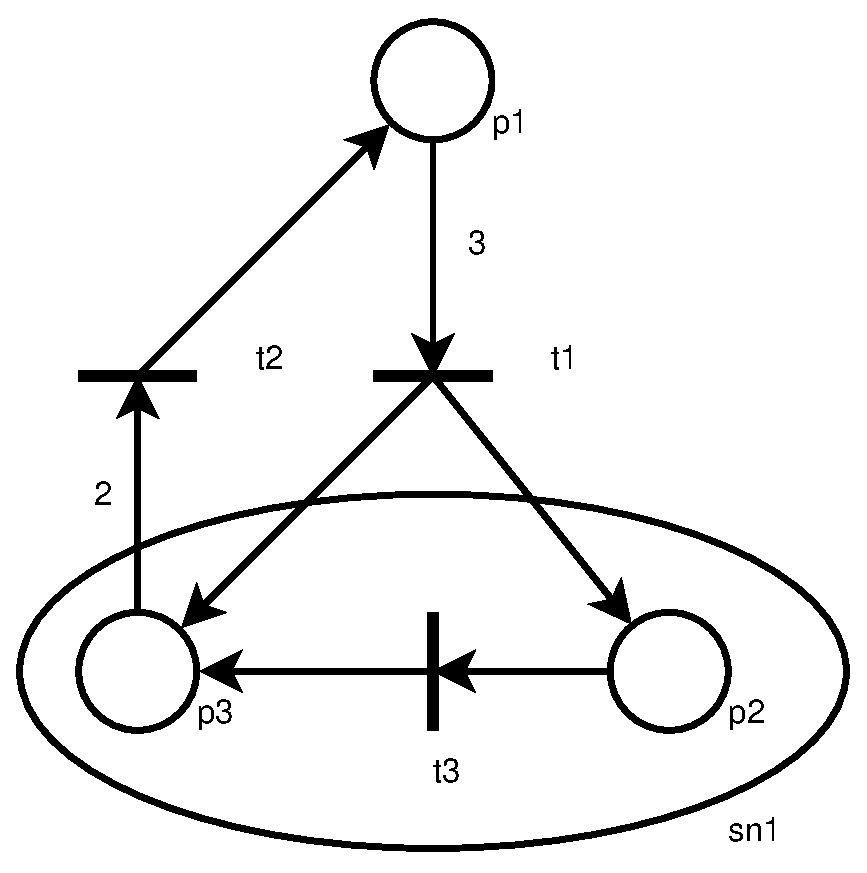
\includegraphics[width=0.40\textwidth]{Figures/PNML-RdPSubred.eps}
\]
\rule{35em}{0.5pt}
 \caption{Subnet to represent in PNML}
 \label{fig:PNML_subnet_to_representRdPSubred}
\end{figure}


The PNML code for this net is:

\begin{lstlisting}
<place id="p1"/>
<place id="p2"/>
<place id="p3"/>
<transition id="t1"/>
<transition id="t2"/>
<transition id="t3"/>
<arc id="a1" source="p1" target="t1">
  <inscription>
    <text> 3 </text>
  </inscription>
</arc>
<arc id="a2" source="t1" target="p2"/>
<arc id="a3" source="t1" target="p3"/>
<arc id="a4" source="p3" target="t2">
  <inscription>
    <text>2</text>
  </inscription>
</arc>
<arc id="a5" source="t3" target="p3"/>
<arc id="a6" source="p2" target="t3"/>
<arc id="a7" source="t2" target="p1"/>
\end{lstlisting}

I want the ellipse region to be a subnet, so I have to specify a subnet with the elements inside the ellipse.



The first step is to define a new tag \texttt{<subnet>}. This tag will have an id, as the rest of PNML elements. And now we proceed
in this way:

\begin{enumerate}
\item The places and transitions inside the subnet are moved into the \textless subnet\textgreater\ tag
\item The arcs joining subnet elements will be included inside the tag
\item The arcs entering or leaving the subnet will be copied inside the tag.
This mean that there are arcs duplicated inside and outside the tag
\end{enumerate}


If we apply these rules to the example:

\begin{enumerate}
\item $p2$, $p3$ and $t3$ are moved into the tag \texttt{<subnet>}
\item $a5$ and $a6$ are put inside the tag
\item $a2$, $a3$ and $a4$ are copied inside the tag
\end{enumerate}

and we have this other PNML extended code: 

\begin{lstlisting}
<subnet id="sn1">
  <place id="p2"/>
  <place id="p3"/>
  <transition id="t3"/>
  <arc id="a2" source="t1" target="p2"/>
  <arc id="a3" source="t1" target="p3"/>
  <arc id="a4" source="p3" target="t2">
    <inscription>
      <text> 2 </text>
    </inscription>
  </arc>
  <arc id="a5" source="t3" target="p3"/>
  <arc id="a6" source="p2" target="t3"/>
</subnet>
<place id="p1"/>
<transition id="t1"/>
<transition id="t2"/>
<arc id="a1" source="p1" target="t1">
  <inscription>
    <text> 3 </text>
  </inscription>
</arc>
<arc id="a2" source="t1" target="p2"/>
<arc id="a3" source="t1" target="p3"/>
<arc id="a4" source="p3" target="t2">
  <inscription>
    <text> 2 </text>
  </inscription>
</arc>
<arc id="a7" source="t2" target="p1"/>
\end{lstlisting}

Now this is one of the most important moment in this work: I will separate the inside
and the outside of the subnet completely. Taking advantage of the process described in chapter \ref{Chapter: Subnets}, I have to extract the front-end from this subnet.

In this case I have two igp (input gate to a place) and an ogt (output gate to a transition) with weight 2. The figure \ref{fig:PNML_InterfazSubredEjemplo1} illustrates the interface associated:

\begin{figure}[htbp]
\centering
\[
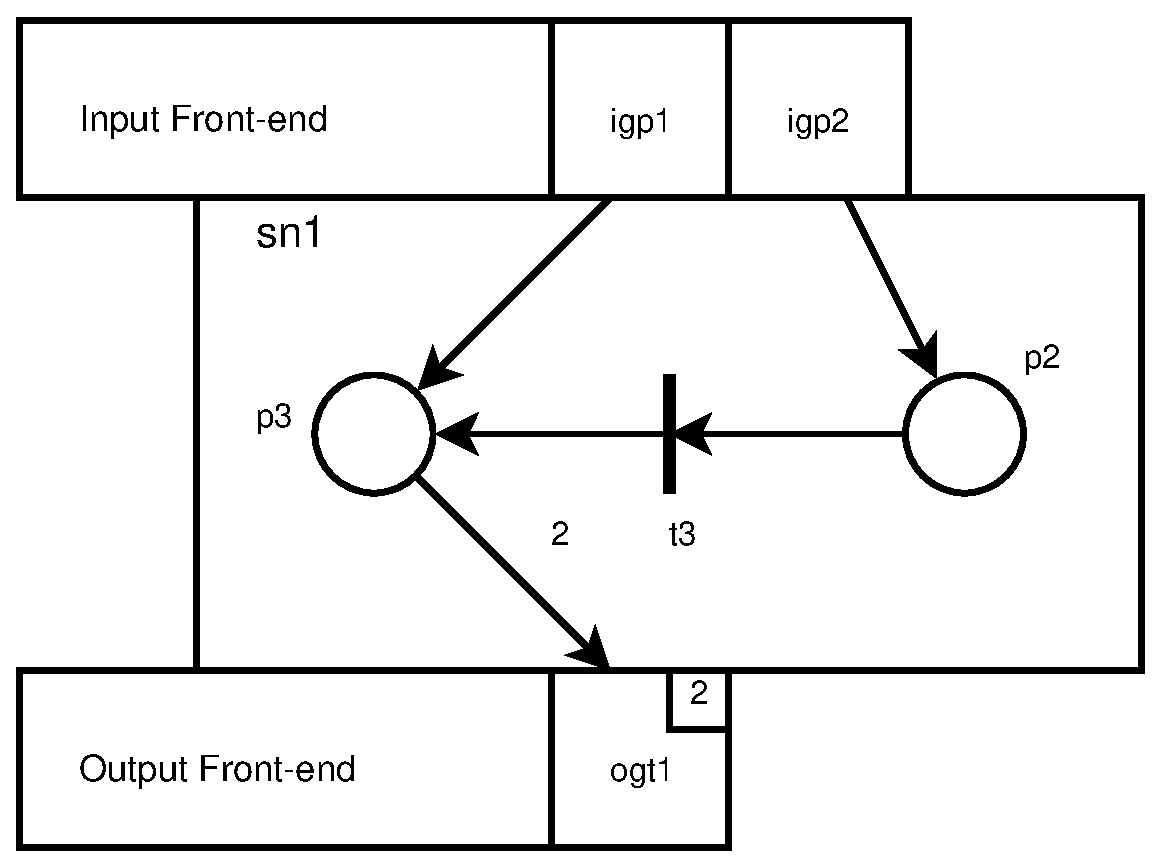
\includegraphics[width=0.50\textwidth]{Figures/PNML-InterfazSubredEjemplo1.eps}
\]
\rule{35em}{0.5pt}
 \caption{Subnet with its interface}
 \label{fig:PNML_InterfazSubredEjemplo1} 
\end{figure}


And the figure \ref{fig:PNML_SubredEjemplo1} is the complete net including the subnet and its front-end

\begin{figure}[htbp]
\centering
\[
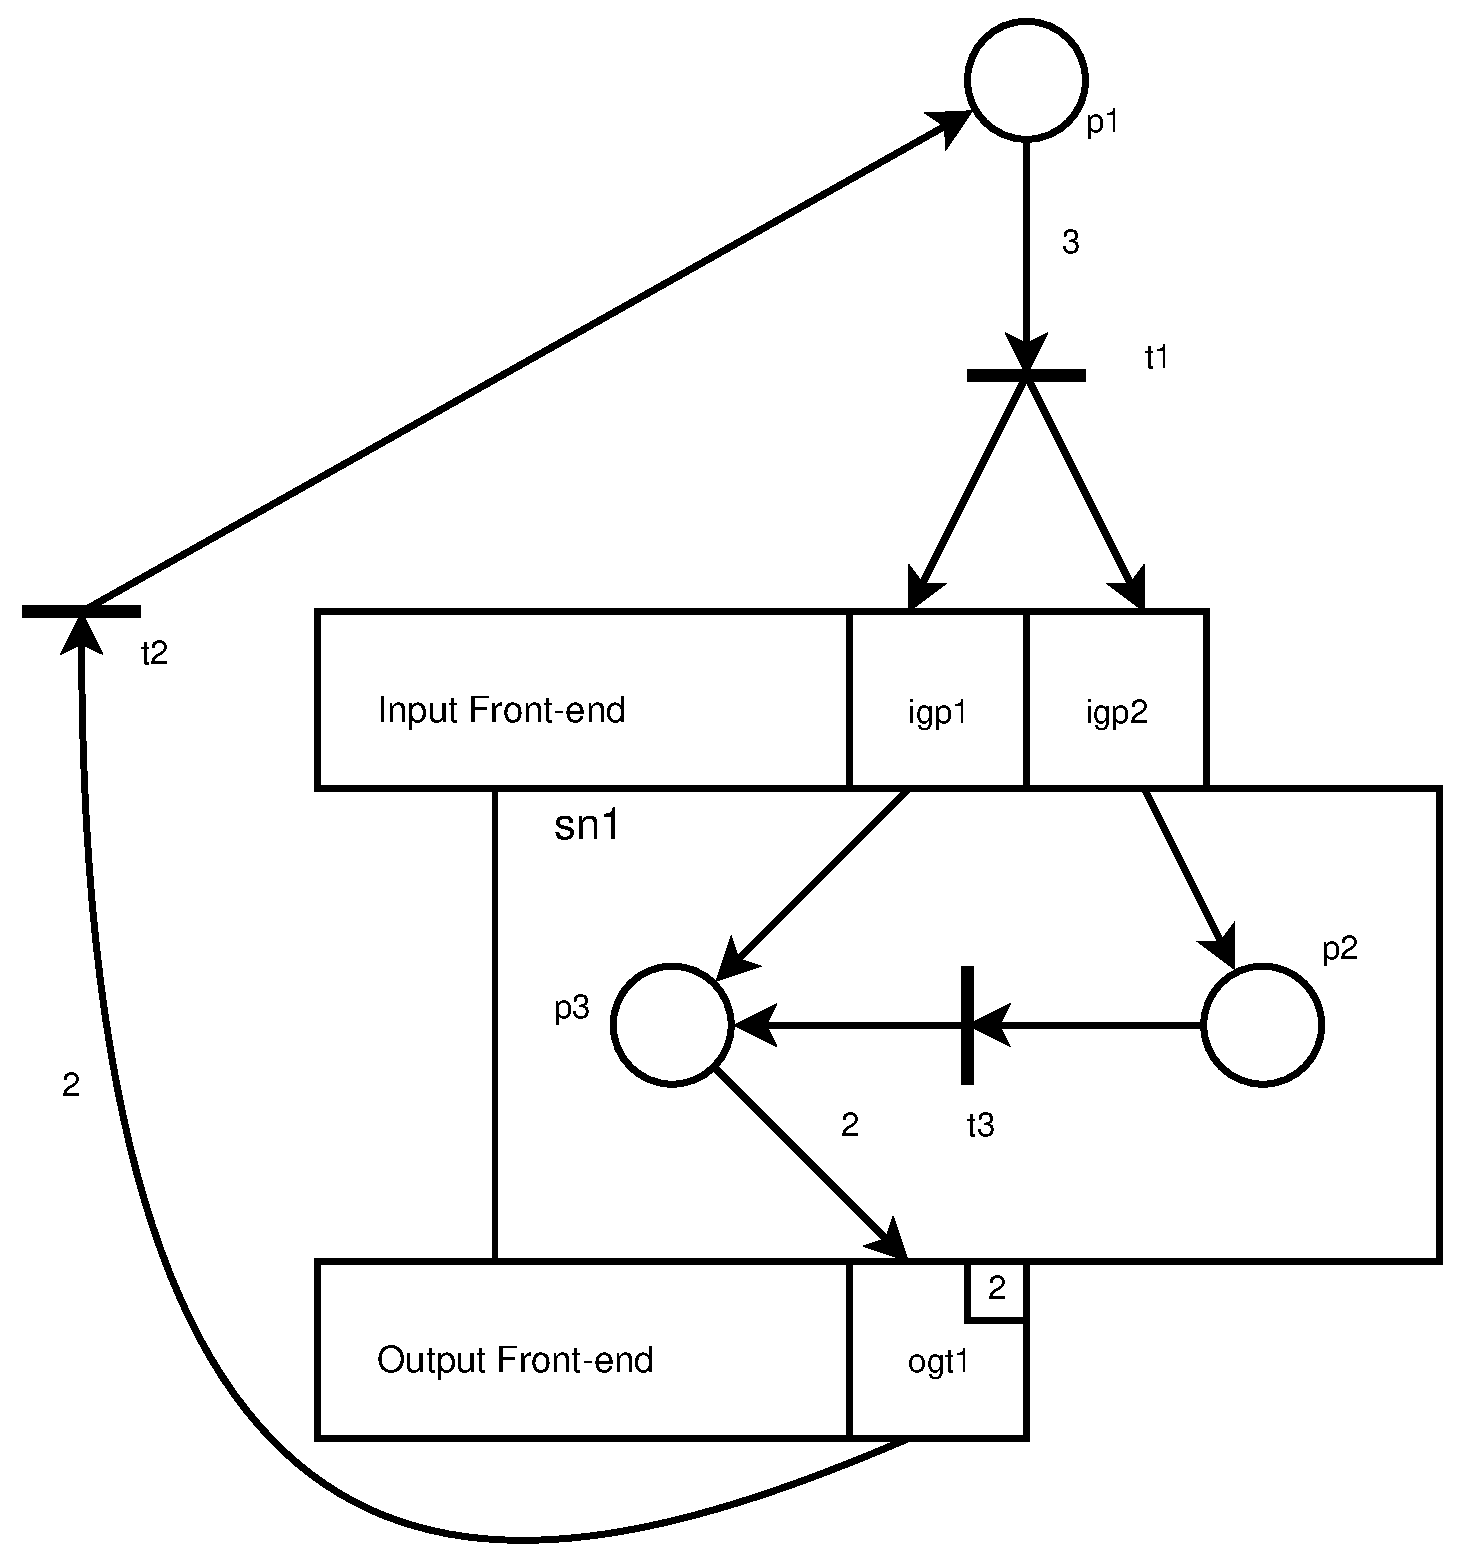
\includegraphics[width=0.60\textwidth]{Figures/PNML-SubredEjemplo1.eps}
\]
\rule{35em}{0.5pt}
 \caption{Petri net with subnet}
 \label{fig:PNML_SubredEjemplo1} 
\end{figure}
 
And now that I have the graphic, how can I represent it in PNML? To answer
this question I will define four new tags: \texttt{<interface>},
\texttt{<gate>}, \texttt{<inscription>} and \texttt{<content>}. Let's explain them.

As its name says, \texttt{<interface>} is
the tag name for encapsulate the front-end. This tag has no attributes (just
the id, of course)
but
it has embedded the gates inside of it. This gates are represented by \texttt{<gate>}. This tag has two new attributes: \texttt{action} and \texttt{type}.
These two attributes have information about the gates. The attribute \texttt{action}
can take two different values: \texttt{input} and \texttt{output}. It indicates
whether the gate is an input gate or an output gate. The other attribute,
\texttt{type}, can take other two values: \texttt{place} and \texttt{transition}.
As arcs have weight, gates have it too. For being in accordance, I define
the tag \texttt{<inscription>} embedded in the tag \texttt{<gate>}. It has the weight of the arc associated.\ 

There is one other tag \texttt{<content>} that
probably at this moment seems useless, but it is necessary for the rest of the process, as we will see in the next chapter. So I am going to introduce it now. This tag is used to encapsulate the rest of the subnet outside the interface. That is, \texttt{<subnet>} has two children:
\texttt{<interface>} and \texttt{<content>},
that have the input/output gates and the rest of the elements, respectively.

Applying this definition to the example, we will have this code

\begin{lstlisting}
<subnet id="sn1">
  <interface id="sn1-interface">
    <gate id="igp1" action="input" type="place"/>
    <gate id="igp2" action="input" type="place"/>
    <gate id="ogt1" action="output" type="transition">
      <inscription>
        <text> 2 </text>
      </inscription>
    </gate>
  </interface>
  <content id="sn1-content">
    <place id="p2"/>
    <place id="p3"/>
    <transition id="t3"/>
    <arc id="a2" source="t1" target="p2"/>
    <arc id="a3" source="t1" target="p3"/>
    <arc id="a4" source="p3" target="t2">
      <inscription>
        <text> 2 </text>
      </inscription>
    </arc>
    <arc id="a5" source="t3" target="p3"/>
    <arc id="a6" source="p2" target="t3"/>
  </content>
</subnet>
<place id="p1"/>
<transition id="t1"/>
<transition id="t2"/>
<arc id="a1" source="p1" target="t1">
  <inscription>
    <text> 3 </text>
  </inscription>
</arc>
<arc id="a2" source="t1" target="p2"/>
<arc id="a3" source="t1" target="p3"/>
<arc id="a4" source="p3" target="t2">
  <inscription>
    <text> 2 </text>
  </inscription>
</arc>
<arc id="a7" source="t2" target="p1"/>
\end{lstlisting}

At this moment I have to do only one thing more. The last step is to modify
the arcs that are repeated inside and outside the net changing their source or target, depending on where is it:

\begin{itemize}
\item If the arc is \textbf{entering} the subnet
  \begin{itemize}
  \item For the \texttt{<arc>} tag inside the tag \texttt{<subnet>}, the \textbf{source} attribute of the arc is changed by the \textbf{input} gate associated
  \item For the \texttt{<arc>} tag outside the tag \texttt{<subnet>}, the \textbf{target} attribute of the arc is changed by the \textbf{output} gate associated
  \end{itemize}
\item If the arc is \textbf{leaving} the subnet
  \begin{itemize}
  \item For the \texttt{<arc>} tag inside the tag \texttt{<subnet>}, the \textbf{target} attribute of the arc is changed by the \textbf{input} gate associated
  \item For the \texttt{<arc>} tag outside the tag \texttt{<subnet>}, the \textbf{source} attribute of the arc is changed by the \textbf{output} gate associated
  \end{itemize}
\end{itemize}

Applying again this rule to the example we have the definitive code for this
Petri net:

\begin{lstlisting}[label=pmnl_final_representation,caption=Final PNML representation]
<subnet id="sn1">
  <interface id="sn1-interface">
    <gate id="igp1" action="input" type="place"/>
    <gate id="igp2" action="input" type="place"/>
    <gate id="ogt1" action="output" type="transition">
      <inscription>
        <text> 2 </text>
      </inscription>
    </gate>
  </interface>
  <content id="sn1-content">
    <place id="p2"/>
    <place id="p3"/>
    <transition id="t3"/>
    <arc id="a2" source="igp2" target="p2"/>
    <arc id="a3" source="igp1" target="p3"/>
    <arc id="a4" source="p3" target="ogt1">
      <inscription>
        <text> 2 </text>
      </inscription>
    </arc>
    <arc id="a5" source="t3" target="p3"/>
    <arc id="a6" source="p2" target="t3"/>
  </content>
</subnet>
<place id="p1"/>
<transition id="t1"/>
<transition id="t2"/>
<arc id="a1" source="p1" target="t1">
  <inscription>
    <text> 3 </text>
  </inscription>
</arc>
<arc id="a2" source="t1" target="igp2"/>
<arc id="a3" source="t1" target="igp1"/>
<arc id="a4" source="ogt1" target="t2">
  <inscription>
    <text> 2 </text>
  </inscription>
</arc>
<arc id="a7" source="t2" target="p1"/>
\end{lstlisting}

Once this is done, the only way to enter or leave the subnet is crossing
the front-end, and I have reached my goal.

This is a comprehensive definition of how to represent subnets in PNML. Now
there are several ways to create a grammar extension that frame this structure
of xml. For example, we can define a dtd file\cite{PNML-dtd}, and xsd file
\cite{PNML-xsd1,PNML-xsd2} or, by coherence with the original grammar of PNML, a Relax NG file \cite{PNML-relaxng.org}. I have defined a way to represent subnets, but the formal grammar is outside the scope of my work because of the wide casuistry of these Petri net types.
However, the method is explained enough on order to each one of these types to define their ox extension. 

 
//TODO gramatica de las subredes para RdP basicas?? Si da tiempo

\subsubsection{Examples of PNML subnets}

Let's take the examples of \ref{fig:Petri_net_examples}. The coloured subnets in the figure \ref{fig:Petri_subnet_examples}  are going to be represented.

\begin{figure}[htbp]
\centering
\[
 \begin{matrix} 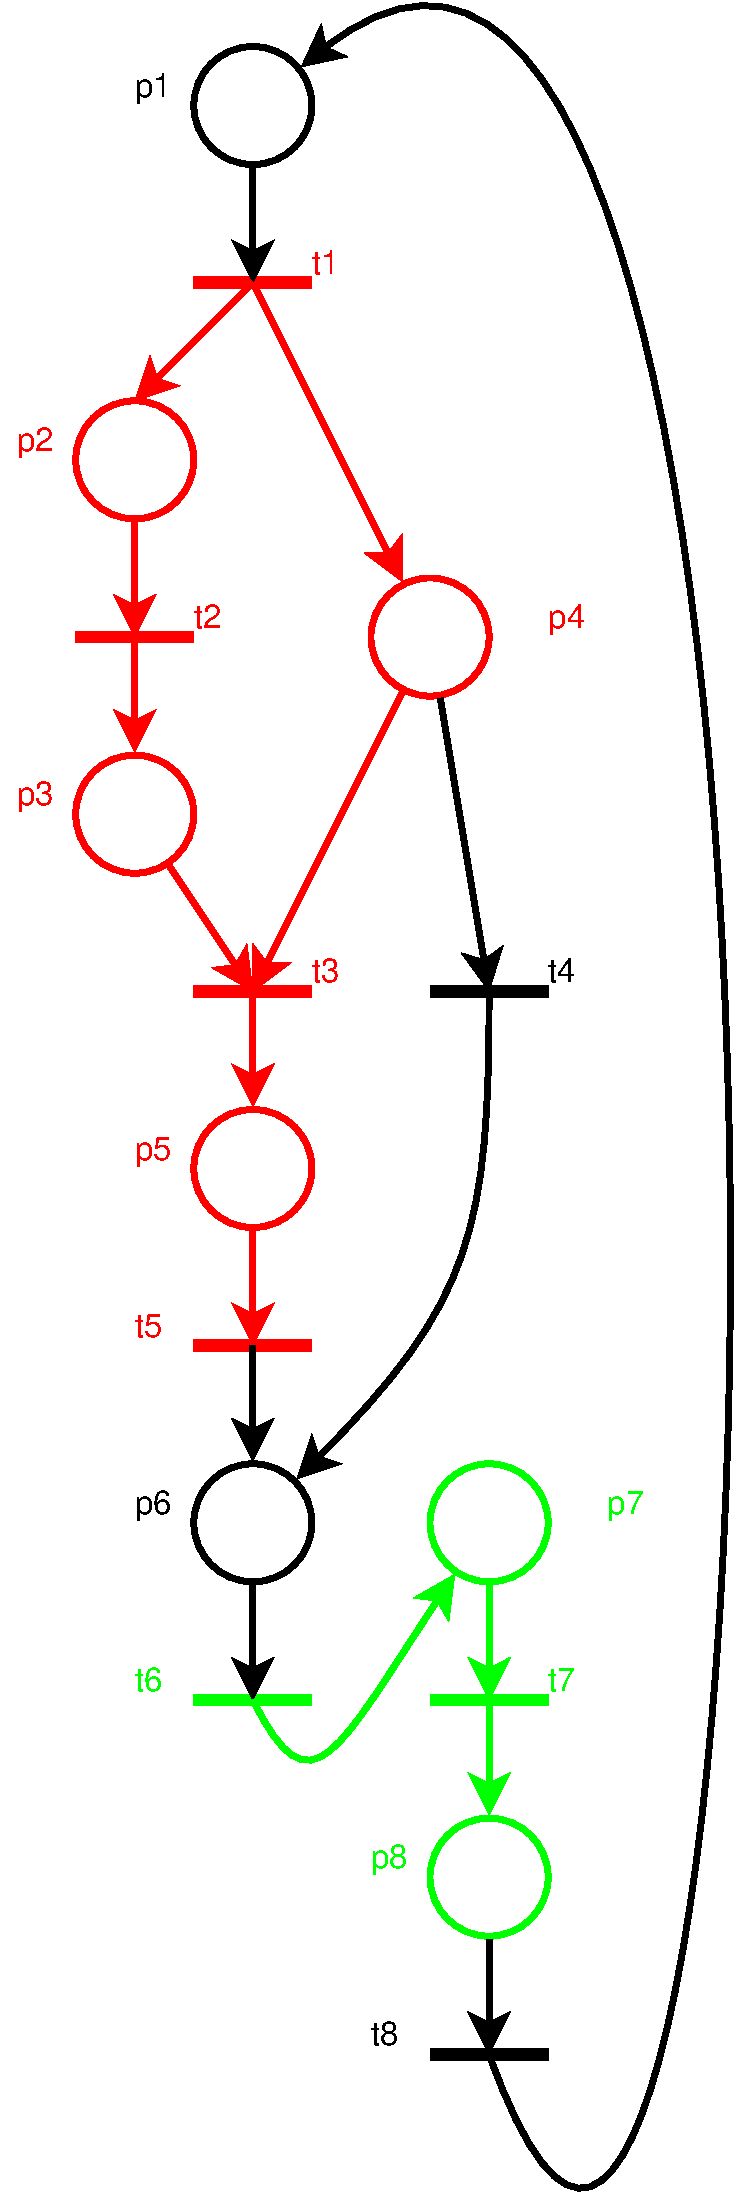
\includegraphics[width=0.2\textwidth]{Figures/PNML-Latorre_1_subnets.eps}\\a)\end{matrix}
  \ \ \ \ \ \ 
 \begin{matrix}  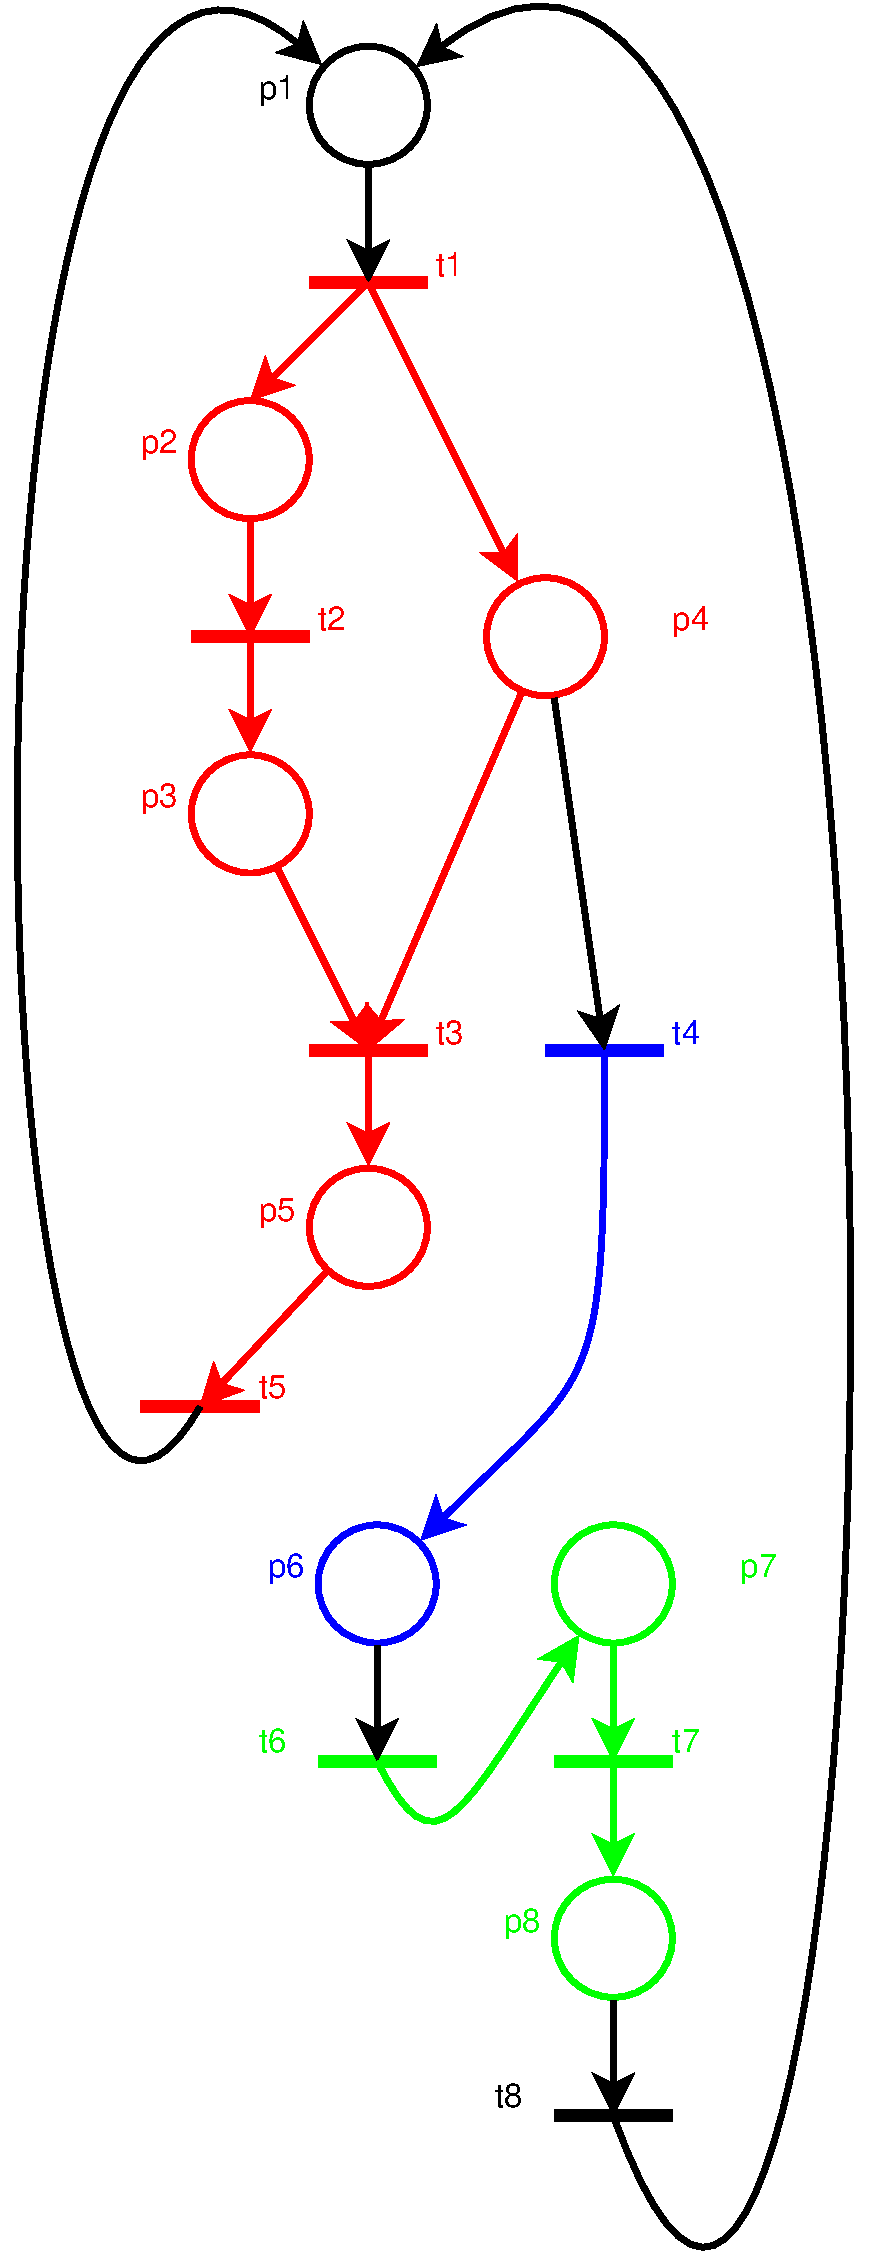
\includegraphics[width=0.23\textwidth]{Figures/PNML-Latorre_2_subnets.eps}\\b)\end{matrix}
  \ \ \ \ \ \ 
 \begin{matrix}  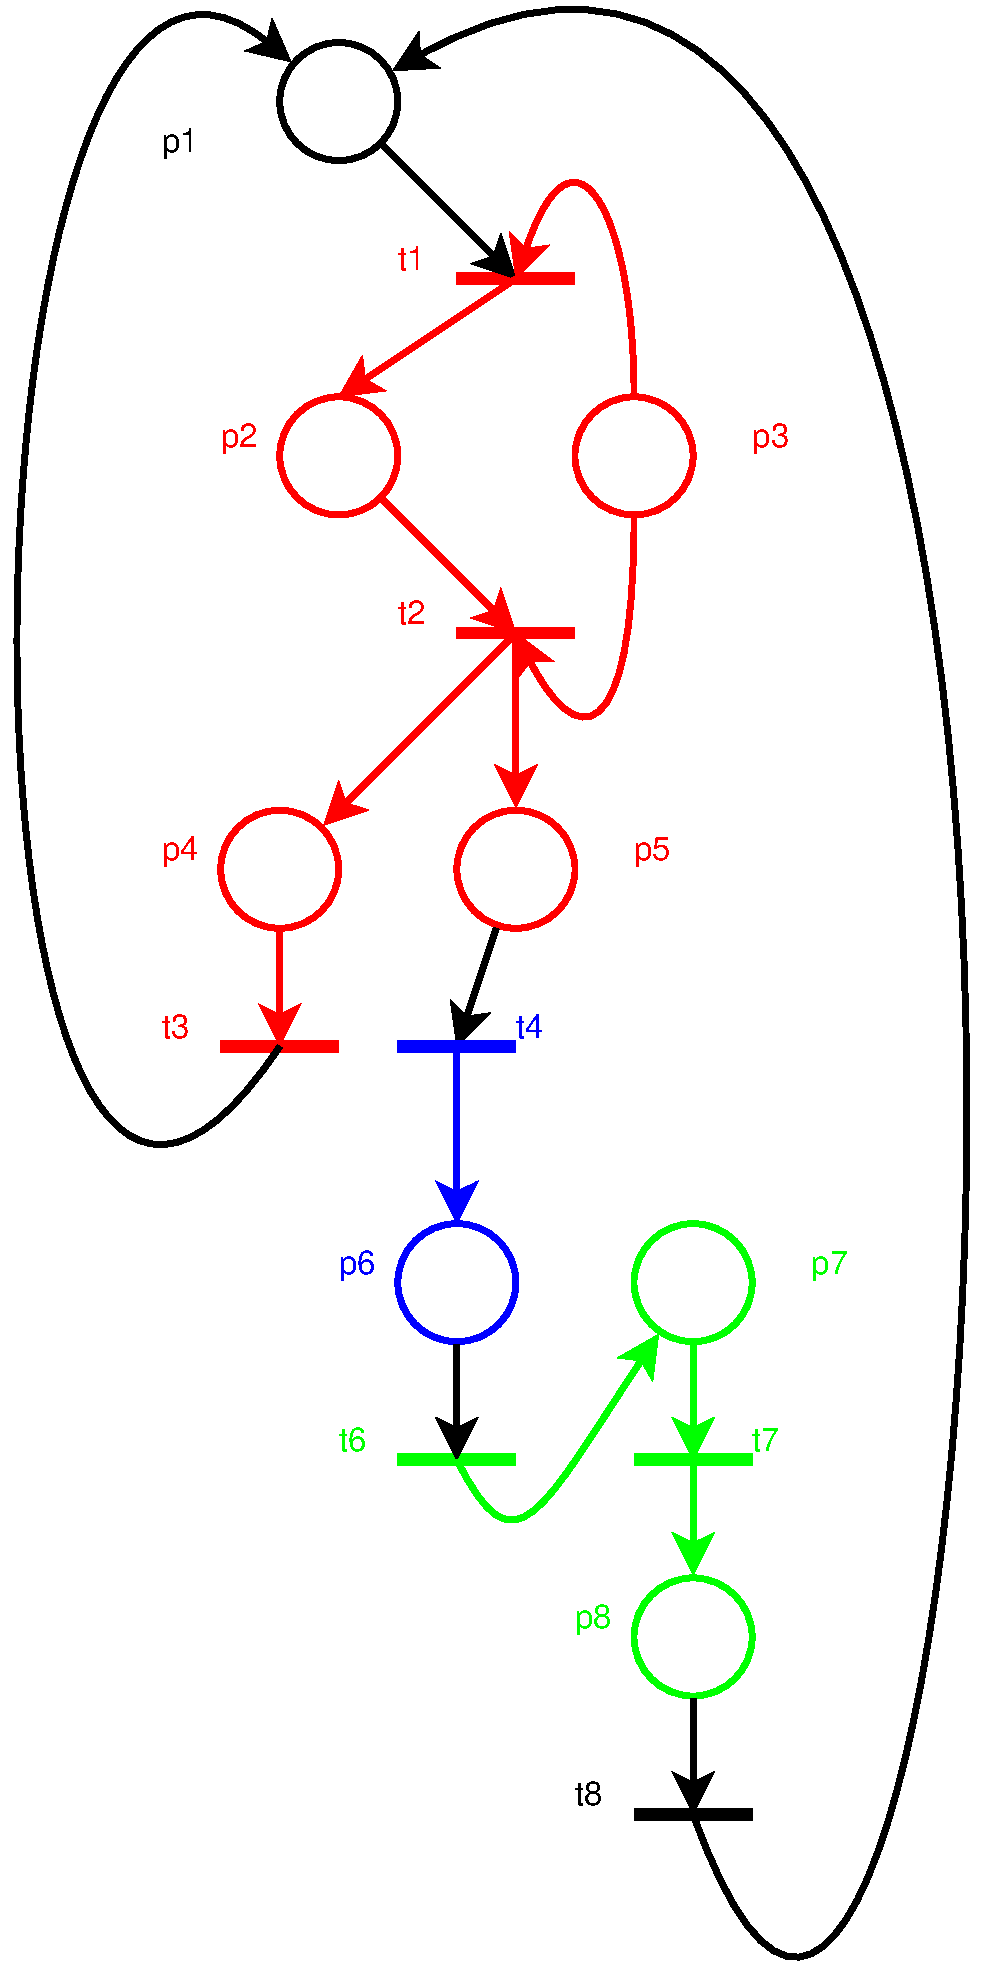
\includegraphics[width=0.3\textwidth]{Figures/PNML-Latorre_3_subnets.eps}\\c)\end{matrix}
\]
\rule{35em}{0.5pt}
 \caption{Three example Petri subnets}
 \label{fig:Petri_subnet_examples} 
\end{figure}

The first net a) is going to be split in two subnets:
\begin{itemize}
\item $N_1$ made up of the places $p_2$, $p_3$, $p_4$ and $p_5$ an the transitions
$t_1$, $t_2$, $t_3$ and $t_5$
\item $N_2$ made up of the places $p_7$ and $p_8$ and the transitions $t_6$
and $t_7$
\item remain outside the subnets the places $p_1$ and $p_6$ and the transitions
%t_4% and $t_8$
\end{itemize}

Let's apply the method explained before.

First, we create two new tags \texttt{<subnet>} with different id with aa
\texttt{<interface>} and a \texttt{<content>} tags inside:

\begin{lstlisting}
<?xml version="1.0" encoding="UTF-8"?>
<pnml
    xmlns="http://www.pnml.org/version-2009/grammar/pnml">
  <net id="latorre1"
      type="http://www.pnml.org/version-2009/grammar/ptnet">
    <page id="page1">
      <subnet id="N1">
        <interface id="N1-interface">
        </interface>
        <content id="N1-content">
        </content>
      </subnet>
      <subnet id="N2">
        <interface id="N1-interface">
        </interface>
        <content id="N2-content">
        </content>
      </subnet>
      <place id="p1"/>
      <place id="p2"/>
      <place id="p3"/>
      <place id="p4"/>
      <place id="p5"/>
      <place id="p6"/>
      <place id="p7"/>
      <place id="p8"/>
      <transition id="t1"/>
      <transition id="t2"/>
      <transition id="t3"/>
      <transition id="t4"/>
      <transition id="t5"/>
      <transition id="t6"/>
      <transition id="t7"/>
      <transition id="t8"/>
      <arc id="a1" source="p1" target="t1"/>
      <arc id="a2" source="t1" target="p2"/>
      <arc id="a3" source="p2" target="t2"/>
      <arc id="a4" source="t2" target="p3"/>
      <arc id="a5" source="t1" target="p4"/>
      <arc id="a6" source="p3" target="t3"/>
      <arc id="a7" source="p4" target="t4"/>
      <arc id="a8" source="p4" target="t3"/>
      <arc id="a9" source="t3" target="p5"/>
      <arc id="a10" source="p5" target="t5"/>
      <arc id="a11" source="t5" target="p6"/>
      <arc id="a12" source="p6" target="t6"/>
      <arc id="a13" source="t6" target="p7"/>
      <arc id="a14" source="p7" target="t7"/>
      <arc id="a15" source="t7" target="p8"/>
      <arc id="a16" source="p8" target="t8"/>
      <arc id="a17" source="t8" target="p1"/>
      <arc id="a18" source="t4" target="p6"/>
    </page>
  </net>
</pnml>
\end{lstlisting}


Now I place their places, transitions and arcs between them inside the correspondent
\texttt{<content>} as shown: 

\begin{lstlisting}
<?xml version="1.0" encoding="UTF-8"?>
<pnml
    xmlns="http://www.pnml.org/version-2009/grammar/pnml">
  <net id="latorre1"
      type="http://www.pnml.org/version-2009/grammar/ptnet">
    <page id="page1">
      <subnet id="N1">
        <interface id="N1-interface">
        </interface>
        <content id="N1_content">
          <place id="p2"/>
          <place id="p3"/>
          <place id="p4"/>
          <place id="p5"/>
          <transition id="t1"/>
          <transition id="t2"/>
          <transition id="t3"/>
          <transition id="t5"/>
          <arc id="a2" source="t1" target="p2"/>
          <arc id="a3" source="p2" target="t2"/>
          <arc id="a4" source="t2" target="p3"/>
          <arc id="a5" source="t1" target="p4"/>
          <arc id="a6" source="p3" target="t3"/>
          <arc id="a8" source="p4" target="t3"/>
          <arc id="a9" source="t3" target="p5"/>
          <arc id="a10" source="p5" target="t5"/>
        </content>
      </subnet>
      <subnet id="N2">
        <interface id="N2-interface">
        </interface>
        <content id="N2_content">
          <place id="p7"/>
          <place id="p8"/>
          <transition id="t6"/>
          <transition id="t7"/>
          <arc id="a13" source="t6" target="p7"/>
          <arc id="a14" source="p7" target="t7"/>
          <arc id="a15" source="t7" target="p8"/>
        </content>
      </subnet>
      <place id="p1"/>
      <place id="p6"/>
      <transition id="t4"/>
      <transition id="t8"/>
      <arc id="a1" source="p1" target="t1"/>
      <arc id="a7" source="p4" target="t4"/>
      <arc id="a11" source="t5" target="p6"/>
      <arc id="a12" source="p6" target="t6"/>
      <arc id="a16" source="p8" target="t8"/>
      <arc id="a17" source="t8" target="p1"/>
      <arc id="a18" source="t4" target="p6"/>
    </page>
  </net>
</pnml>
\end{lstlisting}

Then I define the input and output gates of each subnet. In this case,
I look for the arcs entering or leaving each subnet and the gates that are
defined.

\begin{itemize}
\item The arc $a_1$ is entering $N1$ from a place, so it defines
an $igp$
\item The arc $a_7$ is leaving $N1$ towards a transition, so they defines
an $ogt$
\item The arc $a_{11}$ is leaving $N1$ towards a place, so it defines an
$ogp$
\item The arc $a_{12}$ is entering $N_2$ from a place, so it defines an $igp$
\item The arc $a_{16}$ is leaving $N_2$ towards a transition, so it defines
an $ogt$
\end{itemize}

I put these gates in their location inside the correspondent \texttt{<subnet><interface>}

\begin{lstlisting}
<?xml version="1.0" encoding="UTF-8"?>
<pnml
    xmlns="http://www.pnml.org/version-2009/grammar/pnml">
  <net id="latorre1"
      type="http://www.pnml.org/version-2009/grammar/ptnet">
    <page id="page1">
      <subnet id="N1">
        <interface id="N1-interface">
          <gate id="N1-igp1" action="input" type="place"/>
          <gate id="N1-ogt1" action="output" type="transition"/>
          <gate id="N1-ogp1" action="output" type="place"/>
        </interface>
        <content id="N1_content">
          <place id="p2"/>
          <place id="p3"/>
          <place id="p4"/>
          <place id="p5"/>
          <transition id="t1"/>
          <transition id="t2"/>
          <transition id="t3"/>
          <transition id="t5"/>
          <arc id="a2" source="t1" target="p2"/>
          <arc id="a3" source="p2" target="t2"/>
          <arc id="a4" source="t2" target="p3"/>
          <arc id="a5" source="t1" target="p4"/>
          <arc id="a6" source="p3" target="t3"/>
          <arc id="a8" source="p4" target="t3"/>
          <arc id="a9" source="t3" target="p5"/>
          <arc id="a10" source="p5" target="t5"/>
        </content>
      </subnet>
      <subnet id="N2">
        <interface id="N2-interface">
          <gate id="N2-igp1" action="input" type="place"/>
          <gate id="N2-ogt1" action="output" type="transition"/>
        </interface>
        <content id="N2_content">
          <place id="p7"/>
          <place id="p8"/>
          <transition id="t6"/>
          <transition id="t7"/>
          <arc id="a13" source="t6" target="p7"/>
          <arc id="a14" source="p7" target="t7"/>
          <arc id="a15" source="t7" target="p8"/>
        </content>
      </subnet>
      <place id="p1"/>
      <place id="p6"/>
      <transition id="t4"/>
      <transition id="t8"/>
      <arc id="a1" source="p1" target="t1"/>
      <arc id="a7" source="p4" target="t4"/>
      <arc id="a11" source="t5" target="p6"/>
      <arc id="a12" source="p6" target="t6"/>
      <arc id="a16" source="p8" target="t8"/>
      <arc id="a17" source="t8" target="p1"/>
      <arc id="a18" source="t4" target="p6"/>
    </page>
  </net>
</pnml>
\end{lstlisting}

Then I duplicate the arcs entering or leaving each subnet and change their
source and/or the target for the interface to be an intermediate and their
id in order not to have elements with the same id.

So the figure \ref{fig:PNML_Latorre_1_subnets_interfaces} is the final graphical and PNML representation for de a) net:

\begin{figure}
\[
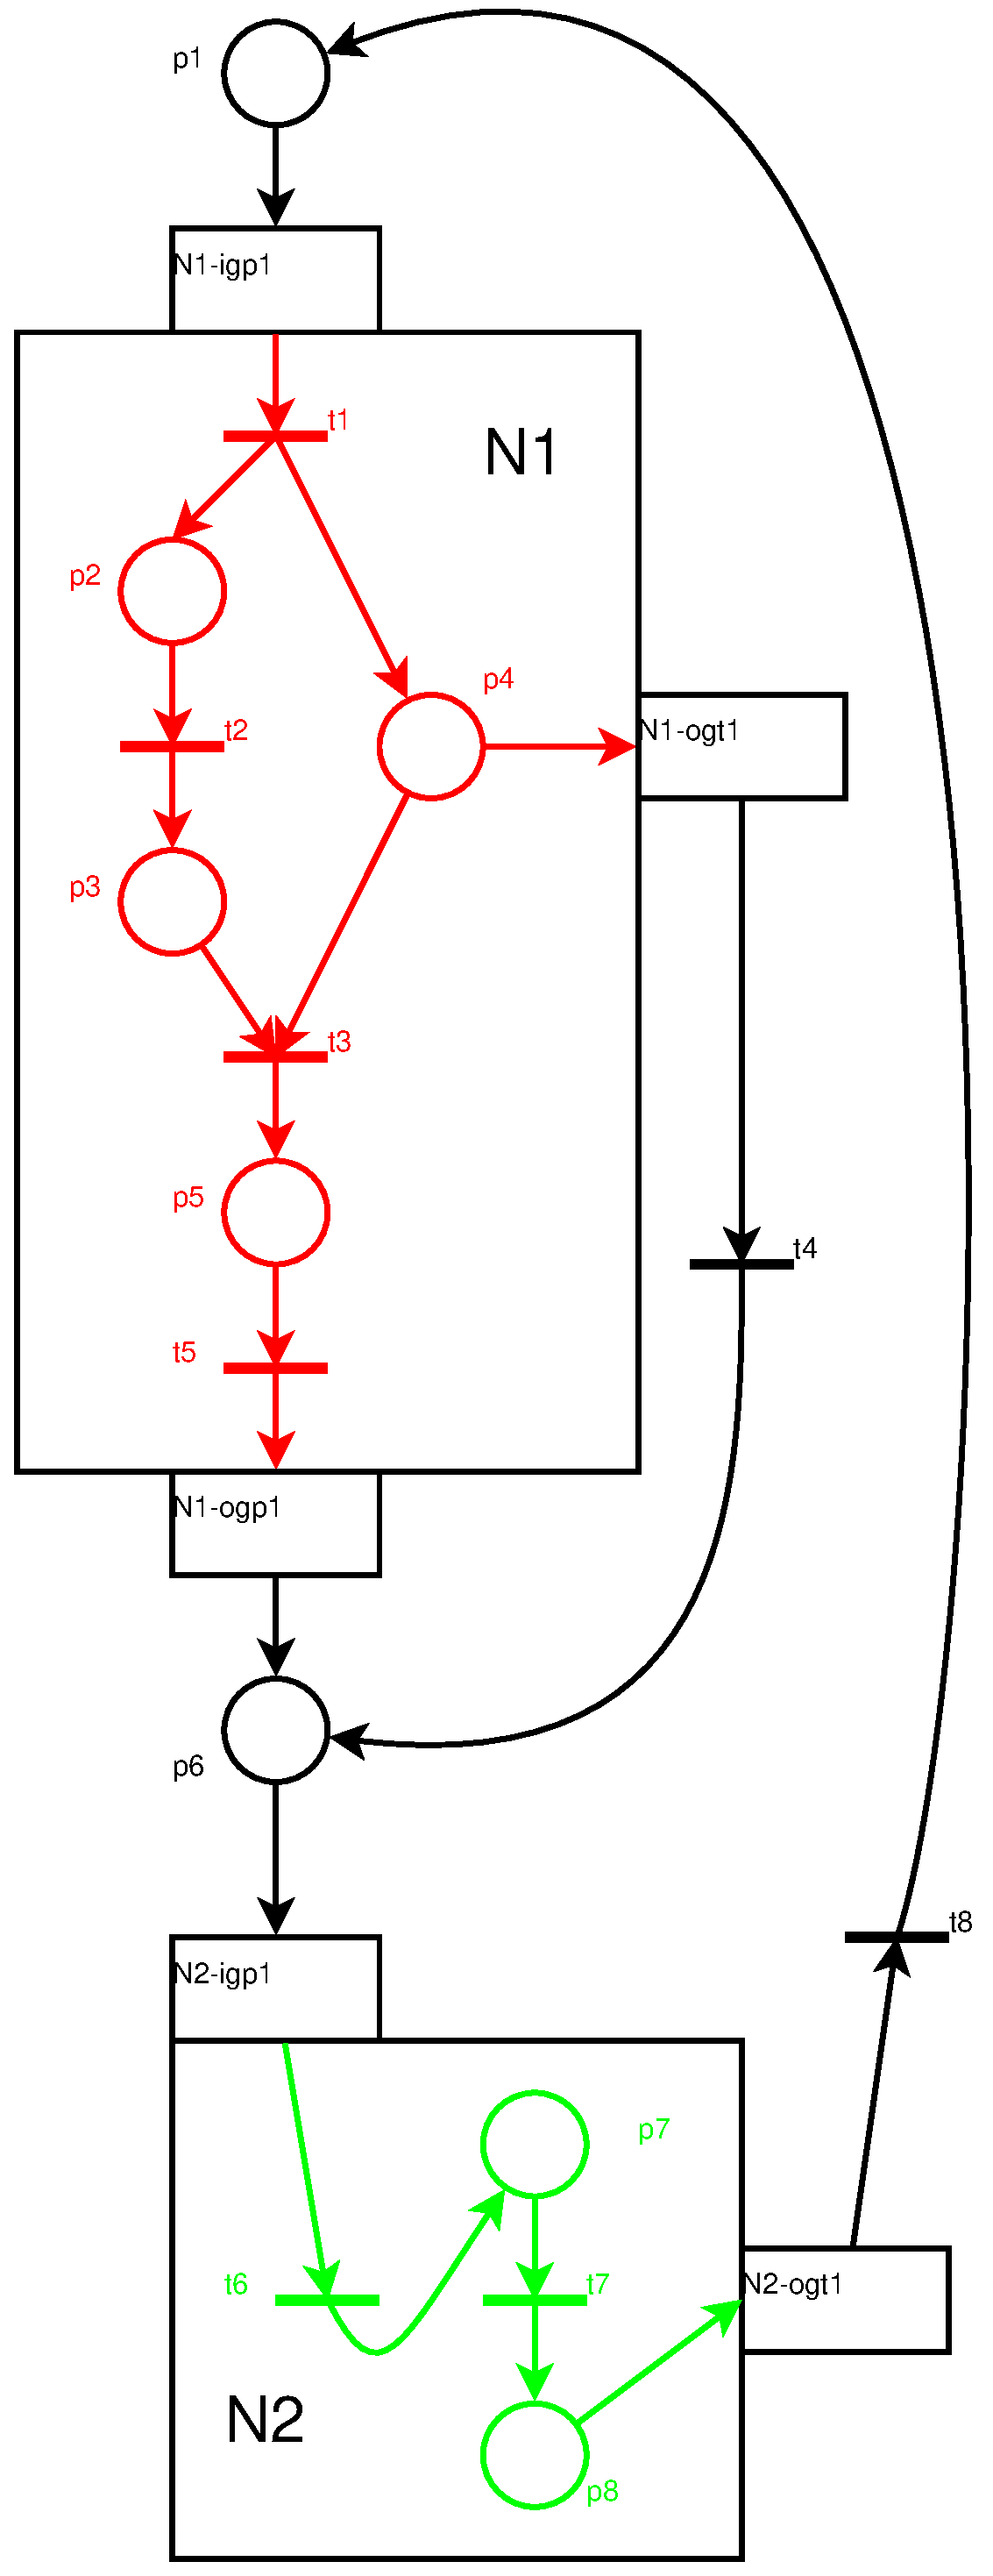
\includegraphics[width=0.35\textwidth]{Figures/PNML-Latorre_1_subnets_interfaces.eps}
\]
\rule{35em}{0.5pt}
 \caption{a) Subnet and interfaces}
 \label{fig:PNML_Latorre_1_subnets_interfaces}
\end{figure} 


\begin{lstlisting}
<?xml version="1.0" encoding="UTF-8"?>
<pnml
    xmlns="http://www.pnml.org/version-2009/grammar/pnml">
  <net id="latorre1"
      type="http://www.pnml.org/version-2009/grammar/ptnet">
    <page id="page1">
      <subnet id="N1">
        <interface id="N1-interface">
          <gate id="N1-igp1" action="input" type="place"/>
          <gate id="N1-ogt1" action="output" type="transition"/>
          <gate id="N1-ogp1" action="output" type="place"/>
        </interface>
        <content id="N1_content">
          <place id="p2"/>
          <place id="p3"/>
          <place id="p4"/>
          <place id="p5"/>
          <transition id="t1"/>
          <transition id="t2"/>
          <transition id="t3"/>
          <transition id="t5"/>
          <arc id="a2" source="t1" target="p2"/>
          <arc id="a3" source="p2" target="t2"/>
          <arc id="a4" source="t2" target="p3"/>
          <arc id="a5" source="t1" target="p4"/>
          <arc id="a6" source="p3" target="t3"/>
          <arc id="a8" source="p4" target="t3"/>
          <arc id="a9" source="t3" target="p5"/>
          <arc id="a10" source="p5" target="t5"/>
          <arc id="N1-a1" source="N1-igp1" target="t1"/>
          <arc id="N1-a7" source="p4" target="N1-ogt1"/>
          <arc id="N1-a11" source="t5" target="N1-ogp1"/>
        </content>
      </subnet>
      <subnet id="N2">
        <interface id="N2-interface">
          <gate id="N2-igp1" action="input" type="place"/>
          <gate id="N2-ogt1" action="output" type="transition"/>
        </interface>
        <content id="N2_content">
          <place id="p7"/>
          <place id="p8"/>
          <transition id="t6"/>
          <transition id="t7"/>
          <arc id="a13" source="t6" target="p7"/>
          <arc id="a14" source="p7" target="t7"/>
          <arc id="a15" source="t7" target="p8"/>
          <arc id="N2-a12" source="N2-igp1" target="t6"/>
          <arc id="N2-a16" source="p8" target="N2-ogt1"/>
        </content>
      </subnet>
      <place id="p1"/>
      <place id="p6"/>
      <transition id="t4"/>
      <transition id="t8"/>
      <arc id="a1" source="p1" target="N1-igp1"/>
      <arc id="a7" source="N1-ogt1" target="t4"/>
      <arc id="a11" source="N1-ogp1" target="p6"/>
      <arc id="a12" source="p6" target="N2-igp1"/>
      <arc id="a16" source="N2-ogt1" target="t8"/>
      <arc id="a17" source="t8" target="p1"/>
      <arc id="a18" source="t4" target="p6"/>
    </page>
  </net>
</pnml>
\end{lstlisting}  


The b) net has three subnets instead of two. The process y the same, but
there is a little difference with a). There are arcs form one output
gate of a subnet to one input gate of other subnet, so an original arc is cut in three parts instead of two. The figure \ref{fig:PNML_Latorre_2_subnets_interfaces} is the graphical result of subnetting

\begin{figure}[htbp]
\[
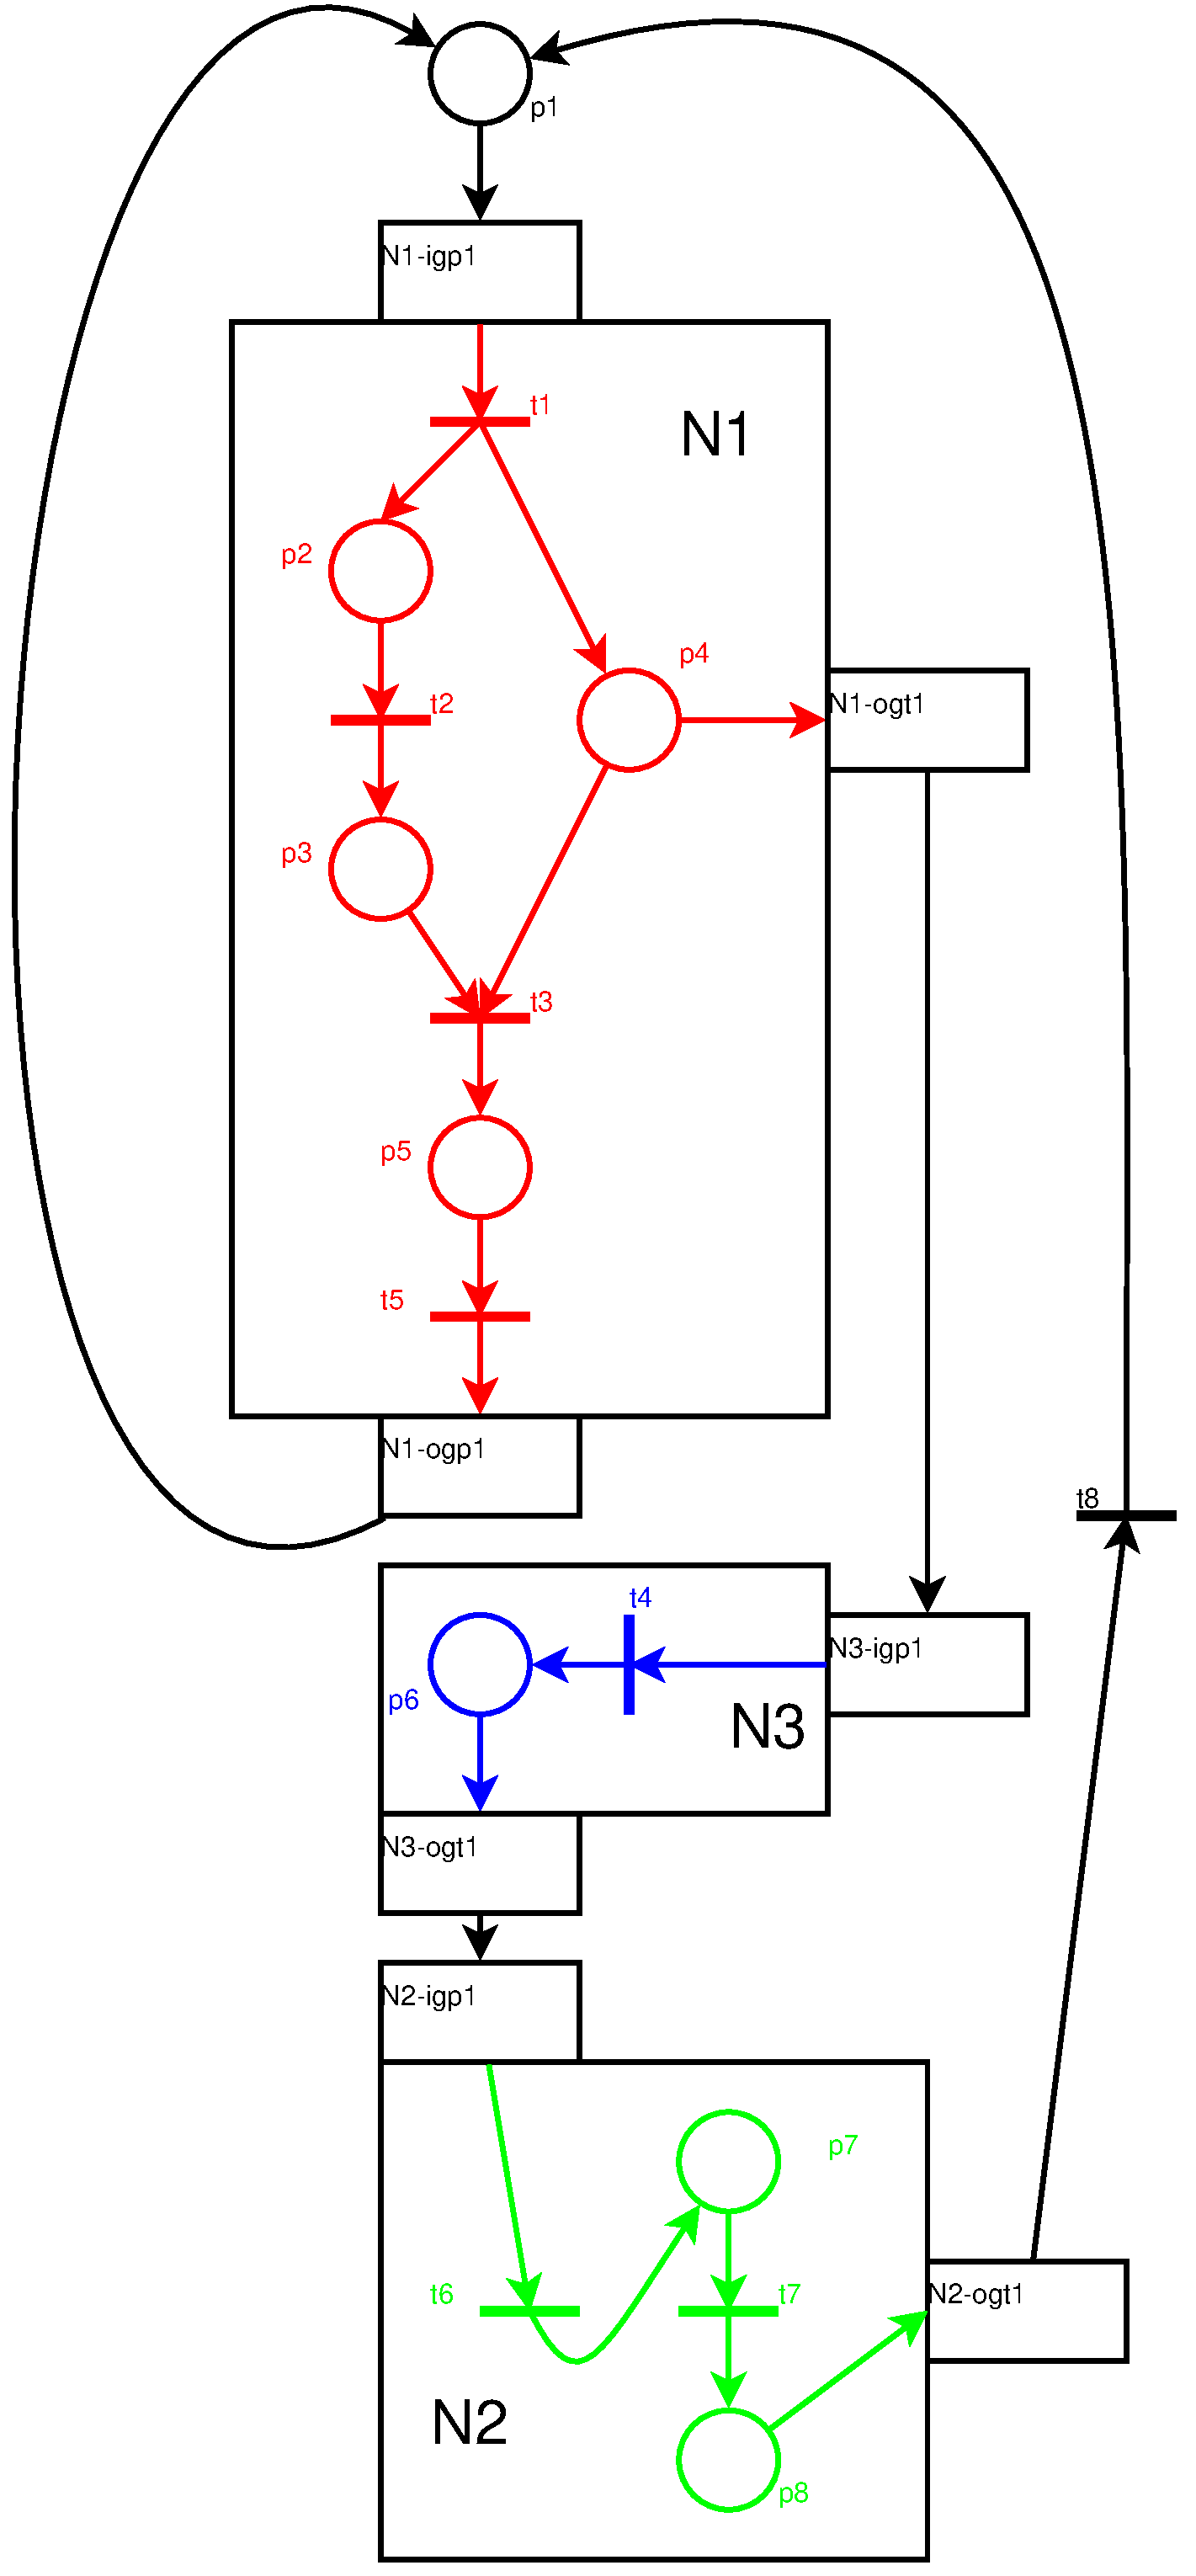
\includegraphics[width=0.35\textwidth]{Figures/PNML-Latorre_2_subnets_interfaces.eps}
\]
\rule{35em}{0.5pt}
 \caption{b) Subnet and interfaces}
 \label{fig:PNML_Latorre_2_subnets_interfaces}
\end{figure} 

And this is the final result of the PNML representation:
\begin{lstlisting}
<?xml version="1.0" encoding="UTF-8"?>
<pnml
    xmlns="http://www.pnml.org/version-2009/grammar/pnml">
  <net id="latorre1"
      type="http://www.pnml.org/version-2009/grammar/ptnet">
    <page id="page1">
      <subnet id="N1">
        <interface id="N1-interface">
          <gate id="N1-igp1" action="input" type="place"/>
          <gate id="N1-ogt1" action="output" type="transition"/>
          <gate id="N1-ogp1" action="output" type="place"/>
        </interface>
        <content id="N1_content">
          <place id="p2"/>
          <place id="p3"/>
          <place id="p4"/>
          <place id="p5"/>
          <transition id="t1"/>
          <transition id="t2"/>
          <transition id="t3"/>
          <transition id="t5"/>
          <arc id="a2" source="t1" target="p2"/>
          <arc id="a3" source="p2" target="t2"/>
          <arc id="a4" source="t2" target="p3"/>
          <arc id="a5" source="t1" target="p4"/>
          <arc id="a6" source="p3" target="t3"/>
          <arc id="a8" source="p4" target="t3"/>
          <arc id="a9" source="t3" target="p5"/>
          <arc id="a10" source="p5" target="t5"/>
          <arc id="N1-a1" source="N1-igp1" target="t1"/>
          <arc id="N1-a7" source="p4" target="N1-ogt1"/>
          <arc id="N1-a11" source="t5" target="N1-ogp1"/>
        </content>
      </subnet>
      <subnet id="N2">
        <interface id="N2-interface">
          <gate id="N2-igp1" action="input" type="place"/>
          <gate id="N2-ogt1" action="output" type="transition"/>
        </interface>
        <content id="N2_content">
          <place id="p7"/>
          <place id="p8"/>
          <transition id="t6"/>
          <transition id="t7"/>
          <arc id="a13" source="t6" target="p7"/>
          <arc id="a14" source="p7" target="t7"/>
          <arc id="a15" source="t7" target="p8"/>
          <arc id="N2-a12" source="N2-igp1" target="t6"/>
          <arc id="N2-a16" source="p8" target="N2-ogt1"/>
        </content>
      </subnet>
      <subnet id="N3">
        <interface id="N3-interface">
          <gate id="N3-igp1" action="input" type="place"/>
          <gate id="N3-ogt1" action="output" type="transition"/>
        </interface>
        <content id="N3_content">
          <place id="p6"/>
          <transition id="t4"/>
          <arc id="N3-a18" source="t4" target="p6"/>
        </content>
      </subnet>
      <place id="p1"/>
      <place id="p6"/>
      <transition id="t4"/>
      <transition id="t8"/>
      <arc id="a1" source="p1" target="N1-igp1"/>
      <arc id="a7" source="N1-ogt1" target="N3-igp1"/>
      <arc id="a11" source="N1-ogp1" target="p1"/>
      <arc id="a12" source="N3-ogt1" target="N2-igp1"/>
      <arc id="a16" source="N2-ogt1" target="t8"/>
      <arc id="a17" source="t8" target="p1"/>
    </page>
  </net>
</pnml>
\end{lstlisting}

The last example is the c) net. It is going to be cut in three subnets too.
The graphical result is the figure \ref{fig:PNML_Latorre_3_subnets_interfaces}:

\begin{figure}[htbp]
\[
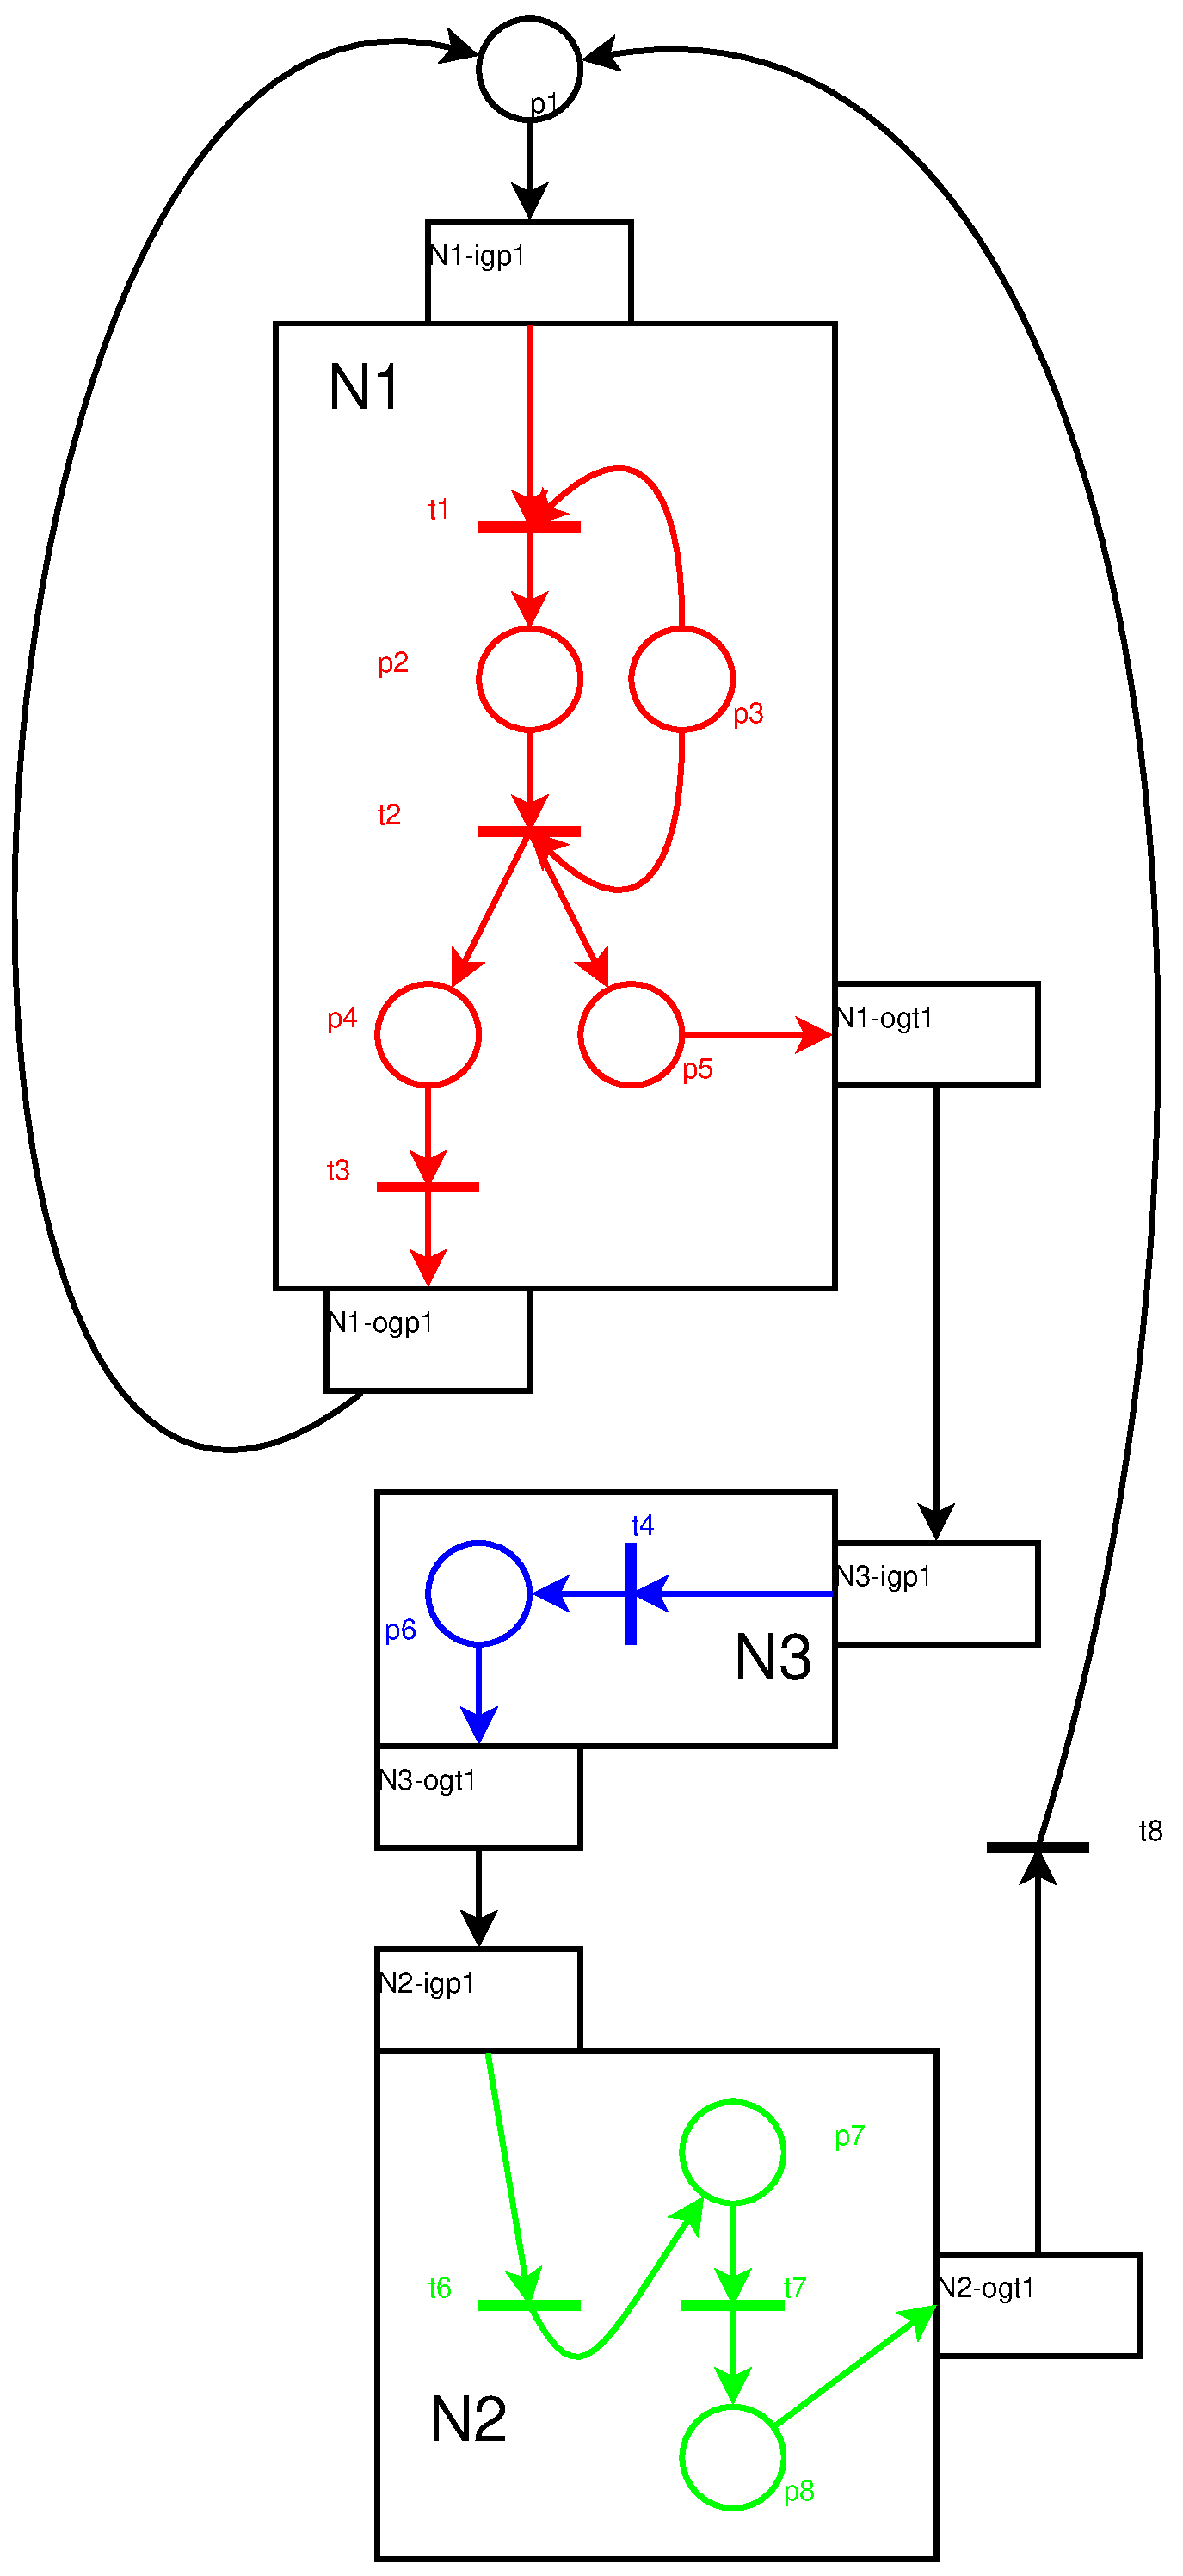
\includegraphics[width=0.4 \textwidth]{Figures/PNML-Latorre_3_subnets_interfaces.eps}
\]
\rule{35em}{0.5pt}
 \caption{c) Subnet and interfaces}
 \label{fig:PNML_Latorre_3_subnets_interfaces}
\end{figure} 

And the PNML representation is:
\begin{lstlisting}
<?xml version="1.0" encoding="UTF-8"?>
<pnml
    xmlns="http://www.pnml.org/version-2009/grammar/pnml">
  <net id="latorre1"
      type="http://www.pnml.org/version-2009/grammar/ptnet">
    <page id="page1">
      <subnet id="N1">
        <interface id="N1-interface">
          <gate id="N1-igp1" action="input" type="place"/>
          <gate id="N1-ogt1" action="output" type="transition"/>
          <gate id="N1-ogp1" action="output" type="place"/>
        </interface>
        <content id="N1_content">
          <place id="p2"/>
          <place id="p3"/>
          <place id="p4"/>
          <place id="p5"/>
          <transition id="t1"/>
          <transition id="t2"/>
          <transition id="t3"/>
          <arc id="a2" source="t1" target="p2"/>
          <arc id="a3" source="p2" target="t2"/>
          <arc id="a4" source="t2" target="p3"/>
          <arc id="a5" source="t1" target="p4"/>
          <arc id="a6" source="p3" target="t3"/>
          <arc id="a8" source="p4" target="t3"/>
          <arc id="a9" source="t3" target="p5"/>
          <arc id="a10" source="p5" target="t5"/>
          <arc id="N1-a1" source="N1-igp1" target="t1"/>
          <arc id="N1-a7" source="p4" target="N1-ogt1"/>
          <arc id="N1-a11" source="t5" target="N1-ogp1"/>
        </content>
      </subnet>
      <subnet id="N2">
        <interface id="N2-interface">
          <gate id="N2-igp1" action="input" type="place"/>
          <gate id="N2-ogt1" action="output" type="transition"/>
        </interface>
        <content id="N2_content">
          <place id="p7"/>
          <place id="p8"/>
          <transition id="t6"/>
          <transition id="t7"/>
          <arc id="a13" source="t6" target="p7"/>
          <arc id="a14" source="p7" target="t7"/>
          <arc id="a15" source="t7" target="p8"/>
          <arc id="N2-a12" source="N2-igp1" target="t6"/>
          <arc id="N2-a16" source="p8" target="N2-ogt1"/>
        </content>
      </subnet>
      <subnet id="N3">
        <interface id="N3-interface">
          <gate id="N3-igp1" action="input" type="place"/>
          <gate id="N3-ogt1" action="output" type="transition"/>
        </interface>
        <content id="N3_content">
          <place id="p6"/>
          <transition id="t4"/>
          <arc id="N3-a18" source="t4" target="p6"/>
        </content>
      </subnet>
      <place id="p1"/>
      <place id="p6"/>
      <transition id="t4"/>
      <transition id="t8"/>
      <arc id="a1" source="p1" target="N1-igp1"/>
      <arc id="a7" source="N1-ogt1" target="N3-igp1"/>
      <arc id="a11" source="N1-ogp1" target="p1"/>
      <arc id="a12" source="N3-ogt1" target="N2-igp1"/>
      <arc id="a16" source="N2-ogt1" target="t8"/>
      <arc id="a17" source="t8" target="p1"/>
    </page>
  </net>
</pnml>
\end{lstlisting}

Note that the interfaces are exactly equals than the b) net. N2 and N3 are
the same, but N1 is different, but with the same interface (attachable net). So I could replace one subnet for another with no problem.

\section{Conclusions}

In this section  we have seen a way to represent subnets in PNML format.
It has not been a formal definition, but general guidelines in order to make
a more extended study of the Petri nets. There are lots of different Petri net types. Each one of them has their own particularities that have to be translated into the PNML format. The method explained here is based on the
basic general Petri nets, but it can see viewed as an algorithm that allow these types to define their own tags. 

Basically, for new xml tags are introduced

\begin{itemize}
\item \texttt{<subnet>} for delimitate the scope (places
and transitions) of the subnet
\item 
\texttt{<interface>} for define the gates to enter or leave the
subnet. Each arc entering or leaving the subnet is associated to a specific
gate. Each gate is represented with the tag \texttt{<gate>} and
can be of several types: input/output (depending on if the arcs enters or
leaves the subnet) and place/transition (depending on
if the arc is associated to a place or a transition inside the subnet)
\item \texttt{<content>} where the places and transitions
inside the subnet are placed, in addition to the arcs between them. \end{itemize} 

The really important thing in this chapter is to identify the subnet and process it in order to extract and interface that is the only way to enter and leave the subnet. The details of each one of the different Petri net types are not specified because of the big casuistry of them.

Once the method is applied, there has to be one subnet content and one subnet interface. There two rules that must be accomplished:

\begin{enumerate}
\item no arc can join nodes inside the subnet with nodes outside and viceversa
\item the interface has to support all the arcs entering and leaving the
subnet with the same information of the arcs that it replace.  
\end{enumerate} If these two rules are complied, then the subnet is correctly
defined. Obviously, this method can be applied several times in order to declare several subnets. the only restriction is that each place or transition can be only in one subnet: no place/transition can be stored in two or more  
